\documentclass[12pt,a4paper,bibliography=totocnumbered,listof=totocnumbered]{scrartcl}
\usepackage[english]{babel}
\usepackage[utf8]{inputenc}
\usepackage{amsmath}
\usepackage{amsfonts}
\usepackage{amssymb}
\usepackage{graphicx}
\usepackage{fancyhdr}
\usepackage{tabularx}
\usepackage{geometry}
\usepackage{setspace}
\usepackage[right]{eurosym}
\usepackage[printonlyused]{acronym}
\usepackage{subfig}
\usepackage{floatflt}
\usepackage[usenames,dvipsnames]{color}
\usepackage{colortbl}
\usepackage{paralist}
\usepackage{array}
\usepackage{titlesec}
\usepackage{parskip}
\usepackage[right]{eurosym}

\usepackage[subfigure,titles]{tocloft}
\usepackage[pdfpagelabels=true]{hyperref}

\usepackage{listings}
\lstset{basicstyle=\footnotesize, captionpos=b, breaklines=true, showstringspaces=false, tabsize=2, frame=lines, numbers=left, numberstyle=\tiny, xleftmargin=2em, framexleftmargin=2em}
\makeatletter
\def\l@lstlisting#1#2{\@dottedtocline{1}{0em}{1em}{\hspace{1,5em} Lst. #1}{#2}}
\makeatother

\geometry{a4paper, top=27mm, left=30mm, right=20mm, bottom=35mm, headsep=10mm, footskip=12mm}

\def \VarAuthor {Simon Danisch}
\def \VarTopic {Romeo: Scripting Environment with interactive Visualizations}

\hypersetup{unicode=false, pdftoolbar=true, pdfmenubar=true, pdffitwindow=false, pdfstartview={FitH},
	pdfauthor={\VarAuthor},
	pdfsubject={\VarTopic},
	pdfcreator={\LaTeX\ with package \flqq hyperref\frqq},
	pdfproducer={pdfTeX \the\pdftexversion.\pdftexrevision},
	pdfkeywords={Bachelor Thesis},
	pdfnewwindow=true,
	colorlinks=true,linkcolor=black,citecolor=black,filecolor=magenta,urlcolor=black}
\pdfinfo{/CreationDate (D:20110620133321)}

\begin{document}

\titlespacing{\section}{0pt}{12pt plus 4pt minus 2pt}{-6pt plus 2pt minus 2pt}

% Kopf- und Fusszeile
\renewcommand{\sectionmark}[1]{\markright{#1}}
\renewcommand{\leftmark}{\rightmark}
\pagestyle{fancy}
\lhead{}
\chead{}
\rhead{\thesection\space\contentsname}
\lfoot{\VarTopic }
\cfoot{}
\rfoot{\ \linebreak Seite \thepage}
\renewcommand{\headrulewidth}{0.4pt}
\renewcommand{\footrulewidth}{0.4pt}

% Vorspann
\renewcommand{\thesection}{\Roman{section}}
\renewcommand{\theHsection}{\Roman{section}}
\pagenumbering{Roman}

% ----------------------------------------------------------------------------------------------------------
% Title Page
% ----------------------------------------------------------------------------------------------------------
\thispagestyle{empty}
\begin{center}
    
\includegraphics[scale=0.5]{graphics/uni.png}\\
    \vspace*{2cm}
    \Large
    \textbf{Faculty of}\\
    \textbf{Cognitive Science}\\
    \vspace*{2cm}
    \Huge
    \textbf{Bachelor's Thesis}\\
    \vspace*{0.5cm}
    \large
    \VarTopic \\
    \vspace*{1cm}
    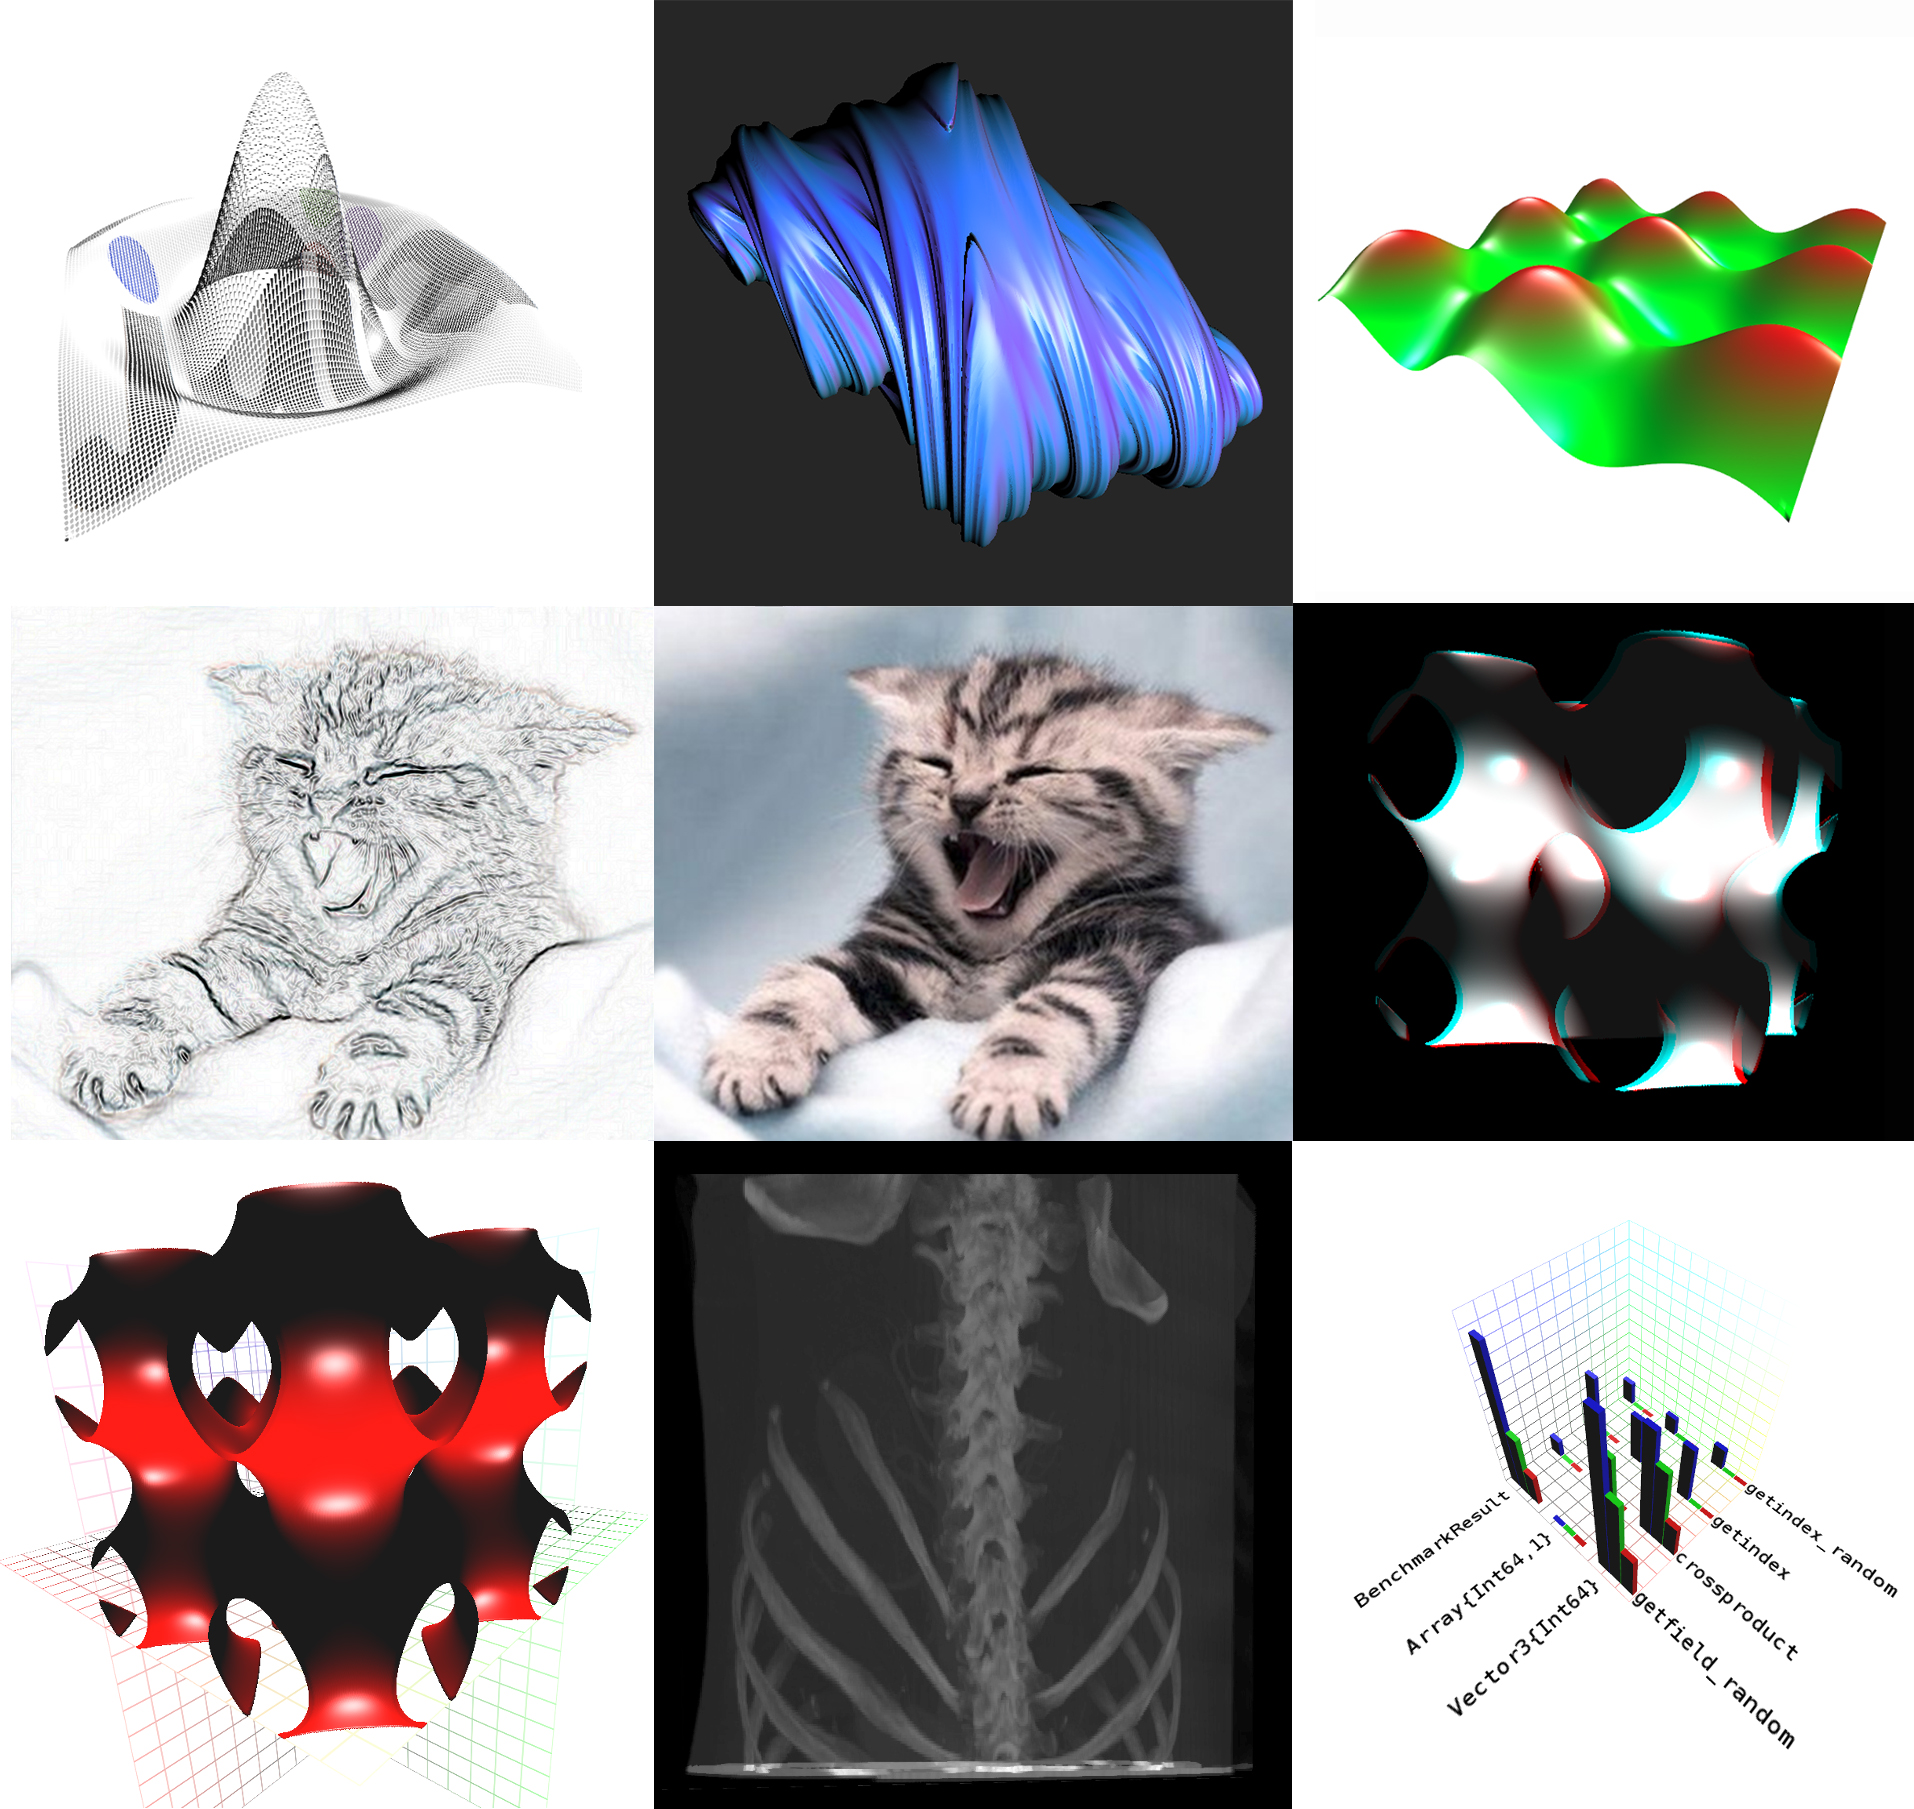
\includegraphics[scale=0.1]{graphics/capabilities.jpg}\\
    \vfill
    \normalsize
    \newcolumntype{x}[1]{>{\raggedleft\arraybackslash\hspace{0pt}}p{#1}}
    \begin{tabular}{x{6cm}p{7.5cm}}
        \rule{0mm}{5ex}\textbf{Author:} & Simon Danisch\newline sdanisch@email.de \\ 
        \rule{0mm}{5ex}\textbf{Supervisor:} & Prof. Dr.-Ing. Elke Pulvermüller \\ 
        \rule{0mm}{5ex}\textbf{Co-Reader:} & Apl. Prof. Dr. Kai-Christoph Hamborg \\ 
        \rule{0mm}{5ex}\textbf{Filing Date:} & 01.02.2014 \\ 
    \end{tabular} 
\end{center}
\pagebreak

% ----------------------------------------------------------------------------------------------------------
% Abstract
% ----------------------------------------------------------------------------------------------------------
\setcounter{page}{1}
\onehalfspacing
\titlespacing{\section}{0pt}{12pt plus 4pt minus 2pt}{2pt plus 2pt minus 2pt}
\rhead{Abstract}
\section{Abstract}
This bachelor thesis introduces Romeo, a prototype for an interactive scripting environment.
Romeo allows the user to execute Julia code and visualize and interact with all variables of the script.
Special care has been taken to make all components easy to use and extendable.
A crucial choice was the programming language, which needs to be both fast and high-level.
Julia is a novel programming language for scientific computing which promises to match the speed of C, while offering a concise coding style. 
This makes Julia a great fit for implementing a scientific visualization library, as speed is crucial for smoothly animated visualizations.
The visualization library, named GLVisualize, was implemented separately from Romeo, to make it usable for similar projects. 
GLVisualize greatest accomplishment is to offer a simple way to animate all data via Signals while offering state of the art performance.
It also offers \ac{GUI} elements, including text fields, sliders and color pickers. 
All libraries are implemented in Julia and the \ac{OpenGL}.
This allows Romeo users to achieve top performance even for large datasets while being able to stay in a high-level language for all tasks.
\pagebreak

% ----------------------------------------------------------------------------------------------------------
% Table of contents
% ----------------------------------------------------------------------------------------------------------
% TODO Typ vor Nummer
\renewcommand{\cfttabpresnum}{Tab. }
\renewcommand{\cftfigpresnum}{Abb. }
\settowidth{\cfttabnumwidth}{Abb. 10\quad}
\settowidth{\cftfignumwidth}{Abb. 10\quad}

\titlespacing{\section}{0pt}{12pt plus 4pt minus 2pt}{2pt plus 2pt minus 2pt}
\singlespacing
\rhead{Table of Contents}
\renewcommand{\contentsname}{II Table of Contents}
\phantomsection
\addcontentsline{toc}{section}{\texorpdfstring{II \hspace{0.35em}Table of Contents}{Table of Contents}}
\addtocounter{section}{1}
\tableofcontents
\pagebreak
\rhead{Listings}
\listoffigures
\pagebreak
\listoftables

\renewcommand{\lstlistlistingname}{Listing}
{\labelsep2cm\lstlistoflistings}
\pagebreak

% ----------------------------------------------------------------------------------------------------------
% Abbreviations
% ----------------------------------------------------------------------------------------------------------
\section{List of Abbreviations}

\begin{acronym}[Acronymes] % längste Abkürzung steht in eckigen Klammern
    \setlength{\itemsep}{-\parsep} % geringerer Zeilenabstand
    \acro{IDE}{Integrated Development Environment}
    \acro{GUI}{Graphical User Interface}
    \acro{LLVM}{Low Level Virtual Machine}
    \acro{IR}{Intermediate Representation}
    \acro{gcc}{GNU Compiler Collection}
    \acro{Matlab}{Matrix Laboratory}
    \acro{REPL}{Read Eval Print Loop}
    \acro{GPU}{Graphics Processing Unit}
    \acro{GLSL}{OpenGL Shading Language}
\end{acronym}



\newpage

% ----------------------------------------------------------------------------------------------------------
% Style
% ----------------------------------------------------------------------------------------------------------
% Abstände Überschrift
\titlespacing{\section}{0pt}{12pt plus 4pt minus 2pt}{-6pt plus 2pt minus 2pt}
\titlespacing{\subsection}{0pt}{12pt plus 4pt minus 2pt}{-6pt plus 2pt minus 2pt}
\titlespacing{\subsubsection}{0pt}{12pt plus 4pt minus 2pt}{-6pt plus 2pt minus 2pt}

% Kopfzeile
\renewcommand{\sectionmark}[1]{\markright{#1}}
\renewcommand{\subsectionmark}[1]{}
\renewcommand{\subsubsectionmark}[1]{}
\lhead{Kapitel \thesection}
\rhead{\rightmark}

\onehalfspacing
\renewcommand{\thesection}{\arabic{section}}
\renewcommand{\theHsection}{\arabic{section}}
\setcounter{section}{0}
\pagenumbering{arabic}
\setcounter{page}{1}


% --------------------------------------------------------------------------
% Introduction
% --------------------------------------------------------------------------
\section{Introduction}
% Just a first sketch:
This Bachelor Thesis is about writing a fast and interactive 3D visualization environment for scientific computing. 
The focus is on usability, applied to all the different interfaces, ranging from abstract API interfaces to graphical user interfaces. 
The ultimate goal is to make scientific computing more accessible to the user.
As \ac{GUI} elements and editable text fields are supplied, one can also write and execute scripts, 
and immediately visualize all bound variables of the script and edit them via simple \ac{GUI} elements like sliders. 
With this it is possible to implement rudimentary interactive programming or visual debugging, further helping the user to understand his algorithms.

The introduction is structured in the following way.
First, an introduction to the general field of research and its challenges is given. 
From these challenges, the problems relevant to this thesis will be extracted.
Finally this chapter will conclude with a solution to the problem, how to measure the success and give an outlook on the structure of the entire Bachelor Thesis.
\subsection{Scientific Computing}
Non professional programmers, using programming as a tool to solve research tasks.
What they want:
Easy to use
Low overhead for small scripts
Fast
Fast and extensible libraries, especiaal for linear algebra
Rich standard library

\subsection{Contribution}
The contribution of this thesis is an interactive visualization library tied to a fast scientific computing language, while entirely written in the same language.

\subsection{Field of Research and Problem}

\vspace{1em}
\begin{minipage}{\linewidth}
    \centering
    
\includegraphics[width=0.7\linewidth]{graphics/surfaces.png}
    \captionof{figure}[Volume Visualization]{different visualizations of $f(x,y,z)=\sin(\frac{x}{15})+\sin(\frac{y}{15})+\sin(\frac{z}{15})$, visualized with Romeo. From left to right: Isosurface with isovalue=0.76, Isosurface with isovalue=0.37, maximum value projection}
    \label{fig:volume}
\end{minipage}
\vspace{1em}

%Scientific computing: visual debugging, interactive programming, high performance
%First rough sketch:
The general research field is making the capabilities of computers more accessible and understandable.
This is a very broad definition and there are many different ways of making it easier to use a computer. 
One of the first big steps was to move from coding in binary to assembly. 
Many more steps have followed, for example introducing graphical user interfaces, novel input devices like the mouse, understandable visualizations and so forth.
All these advances have made computers usable even for people who don't have an education in computer science.
In this bachelor thesis the field is scientific computing, which still has quite a lot of barriers for novel users.
Scientific computing is usually about implementing mathematical equations, complex algorithms and manipulating and analyzing data.
As it is difficult to offer easy to use graphical interfaces for this kind of work, most research is done in some specialized, high-level scientific computing language. As most high-level languages are relatively slow, but for a lot of algorithms state of the art performance is required, this has led to a dual system. Prototyping in a high-level language, and then redoing the work in a fast low-level language.
That this is not the perfect work flow is immediately visible, and a lot of research has been put into making high-level languages faster.
These efforts slowly pay off and there is a whole new range of languages, that claim to be easy to work with while being as fast as it can get.
This is a relatively recent trend and hasn't fully arrived in scientific computing yet, as most languages still have their core implemented in another fast language, which makes it hard to extend them for non professional users.
This is especially true for high performance visualization libraries, which mostly use C++ at their performance critical core.
To leverage the extensibility of these libraries, this bachelor thesis implements a visualization library in a fast high level language.
Visualizations where chosen as they are a crucial building blocks for many fields in scientific computing.

Consider the following function $f(x,y,z)=\sin(\frac{x}{15})+\sin(\frac{y}{15})+\sin(\frac{z}{15})$, which describes a 3D volume mathematically. 
This is a simple function, which is already not that easy to interpret. In figure \ref{fig:volume}, you can see different visualizations of f. 
Especially for more complex functions, visualizing might be the only way to get a deeper understanding of the values that a formula or algorithm produces.
This deeper understanding is crucial for identifying problems in the underlying math, or extending the algorithm.
Additionally, widgets and simple \ac{GUI}s are indispensable, giving scientist an easy way to interact with their data and algorithms.
This helps to further understand the dynamics of the data and quickly spot mistakes.

In summary, the software in this thesis (Romeo) focuses on research which involves writing short scripts, while playing around with some parameters and visualizing the results. 
An example would be a material researcher, who is investigating different 3D shapes and materials and their reaction to pressure.
The researcher would need to read in the 3D object he wants to analyze, have an easy way to tweak the material parameters and it would be preferable to get instant feedback on how the pressure waves propagate through the object.


\subsection{Problem Solutions and Measurements of Success}

All building blocks in this thesis are developed with the purpose in mind to give the user the possibility to visualize and interact with complex 2D and 3D data, while being able to easily extend the library.
To enable this kind of functionality, a lot of parts of the infrastructure need to work seamlessly together.
Certain design choices had to be made to guarantee this. As speed is the most constraining factor, this chapter will start by introducing the design choices that had to be made in order to achieve state of the art speed.

\vspace{1em}
\begin{minipage}{\linewidth}
    \centering
    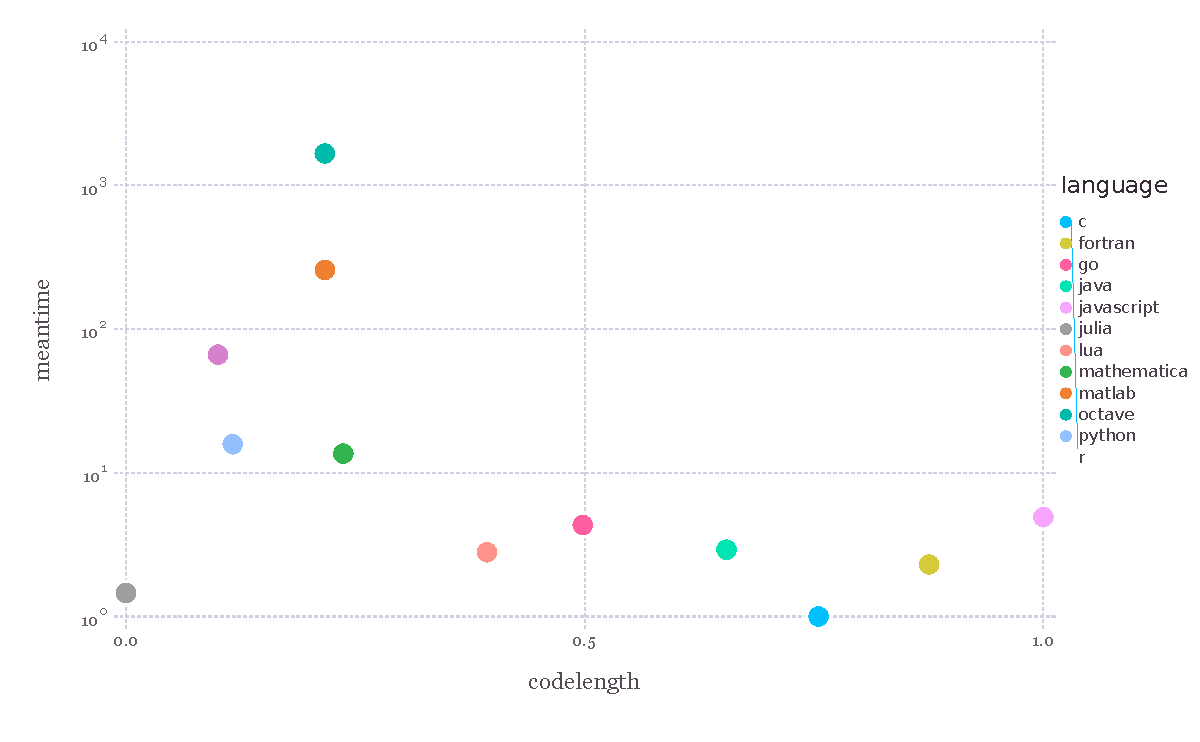
\includegraphics[width=0.9\linewidth]{graphics/julia_bench.pdf}
    \captionof{figure}[Volume Visualization]{Languages speed relative to C (averaged benchmark results), plotted against the length of the needed code (Source in Appendix)}
    \label{fig:juliabench}
\end{minipage}

\subsubsection{Speed}
Speed is mainly a usability factor. It's a factor, that can make a software unusable, or render it unproductive. Because of this, speed has taken a high priority in this thesis. As general coding productivity is also a concern, this thesis is set on using a high level language.
Historically, these two demands can't be both satisfied.
How to achieve state of the art speed with a high level language is an ongoing research and basically the holy grail of language design.
Luckily, there is a new programming language namely Julia building upon the compiler infrastructure \ac{LLVM}, promising a concise, high-level programming style, while approaching C-performance.
This is well illustrated in figure \ref{fig:juliabench}. Code length is an ambiguous measure for conciseness, but if the code is similarly refactored it is a good indicator of how many lines of code need to be written to achieve the same goal.
\ac{LLVM} is an impressive compiler infrastructure, which has front ends for different languages and back-ends for different chip architectures. 
A language designer has the task, to emit \ac{LLVM} \ac{IR}, which than gets just in time compiled and optimized to the architecture resulting in fast machine code.
\ac{LLVM}'s concept is effective, as you can accumulate state of the art optimizations in one place, making them accessible to many languages, while being able to compile to different platforms. There are x86, ARM, OpenCL and CUDA back ends. While Julia doesn't support them all, it will hopefully be possible in the future. 
\ac{LLVM} is also used by Clang, the C/C++ front end for \ac{LLVM} rivaling \ac{gcc} and it is used by Apple's programming language Swift. 
This makes \ac{LLVM} a solid basis for a programming language, as these are highly successful projects guaranteeing \ac{LLVM} further prospering of the technology.
%See table \ref{table:FEComparison}, for a little benchmark.

To get high performant 3D graphics rendering, there are on the first sight a lot of options.
If you start to take the previous demands into account, the options shrink down considerably, though.
The visualization library should be implemented in one high level language, which can be used for scientific computing and has state of the art speed. At this point, there are close to zero libraries left. As you can see in figure \ref{fig:juliabench}, Matlab, Python and R disqualify, as they are too slow. JavaScript, Java, Go and Lua are missing a scientific background and the others are too low level for the described goals.
This leaves only Julia, but in Julia there weren't any 3D libraries available, which means that one has to start from scratch.
There are only a couple of GPU accelerated low-level libraries available, namely Khrono's OpenGL, Microsoft's DirectX, Apple's Metal and AMD's Mantel, which are offering basically the same functionality. As only OpenGL is truly cross-platform, this leaves only OpenGL as an option.
So for the purpose of high speed visualizations, OpenGL was wrapped with a high-level interface written in Julia. This leaves us with one binary dependency not written in Julia, namely the video driver, which implements OpenGL.

Measurement of success is pretty straight forward, but the devil is in the detail.
It's easy to benchmark the code, but quite difficult to find a baseline, as one either has to implement the whole software with the alternative technologies, or one has to find similar software.
This thesis will follow a hybrid strategy, comparing some simple implementations with different technologies and choose some rivaling state of the art libraries as a baseline.

\subsubsection{Extensibility}
Extensibility is an important factor, which can decide, if a library is fit for scientific computing or not. 
It's not only that, but also a great factor determining growth of a software, as the more extensible the software is, the higher the probability that someone else contributes to it.
In order to write extensible software, we first have to clarify what extensibility is.
Extensible foremost needs, that the code is accessible. There are different levels of accessibility. The lowest level is closed source, where people purposely make the code inaccessible. While this is obvious, it is just a special case of not understanding the underlying language. Just shipping binaries without open sourcing the code, means that the source is only accessible in a language which is extremely hard to understand, namely the machine code of the binary. So another example for inaccessibility is to write in a language that is difficult to understand. Other barriers are obfuscated language constructs, missing documentations and cryptic highly optimized code.
Further more the design of the library in the whole is an important factor for extensibility. It's not only important, that all parts are understandable, but also, that every independent unit in the code solves only one problem.
If this is guaranteed, re-usability in different contexts becomes much simpler. This allows for a broader user base, which in turn results in higher contributions and bug reports.
Short concise code is also important, as it will take considerably less time to rewrite something, as the amount of code that has to be touched is shorter and less time is spend on understanding and rewriting the code.

So the code written for this thesis should be open source, modular, written in a high level language and concise.

This is pretty difficult to measure as these are either binary choices, which are either followed or not, 
or higher level concepts like writing concise code, which can be a matter of taste.
To get an idea of the effectiveness of my strategy, usage patterns from github will be analysed.

\subsubsection{Event System}
For interaction events have to be handled. The chosen event system is named Reactive, which also reflects its design principle.
Reactive programming is an event driven approach, using signals as the abstraction. 
Signals are values, which change over time, which can be transformed via functions, yielding a new signal.
Here is an example to clarify the notion of signals:
\begin{lstlisting}
a = Input(40) # an integer signal.
b = Input(2) # an integer signal.
c = lift(+, a,b) # creates a new signal with the value 42
push!(a, 20) # updates a, resulting in c being 22
\end{lstlisting}

The event system was chosen for two reasons:
First, because it simply was the only available event system for Julia at that time.
Secondly, it naturally represents change over time, which is a perfect fit for animations.


\subsubsection{Interfaces}
Working with a computer means working with interfaces to a computer, which in the end simply jiggles around with zeros and ones. There is a huge hierarchy of abstractions involved, to make this process of binary juggling manageable to the human.
We already dealt with the lowest relevant abstraction: the choice of programming language, which forms our first interface to the computer.
The next level of abstraction is the general architecture of the modules, which has been discussed previously. 
This chapter is about the API design choices that have been made.
The first API is the OpenGL layer. The philosophy is to make the wrapper for native libraries as thin and reusable as possible and an one to one mapping of the library itself.
This guarantees re-usability for others, as they might be used to work only with the low-level library and they might disagree with any higher-level abstraction.
Over this sits an abstraction layer needed to simplify the work with OpenGL.
With this abstraction, the actual visualization library is implemented.
APIs for visualization libraries are very difficult to realize, as there are endless ways of visualizing the same data.
The design choice here was to use Julia's rich type system, to better describe the data. 
Julia makes this possible, as you can name the same data differently, without loosing performance.
So you can actually have a unit like meter represented as a native floating point type and have the visualization specialize to this.
Like this you can have a single function e.g. \textit{visualize}, that does creates a default visualization for a lot of common data.
It is parameterizable and can actually be overloaded for different styles.
So the signature looks like this in the end:
\begin{lstlisting}
visualization{data} = visualize(data, style=default, parameters=default)
\end{lstlisting}
The same principle is used for editing data, so there is also:
\begin{lstlisting}
visualization{data}, signal{data} = edit(data, style=default, parameters=default)
\end{lstlisting}
Together with the event system which consists of signals, it is possible to edit and visualize rich data over a simple interface, which is perfect for visual debugging, as it is always the same function call applied to the data and no further user interaction is needed.
It is also easy to extend, as the user just has to overload the function, with a custom style and or parameters.
Finally, there are also graphical user interfaces developed for this thesis. As also optimizing them is out of the scope of this thesis, they are kept very simple.
The measurement of success is again relatively difficult to do. (I need to think this over)

\subsection{Outlook}
%Structure of BA and a few worts on the results 

\subsection{Used Technologies}


\subsection{Similar Work}e


\subsubsection{The Julia Programming Language}
Bringing Julia's ease of use and speed to a dynamic visualization library is the declared goal, which makes Julia a crucial building block for this thesis.
Julia is a multi paradigma language for scientific computing.
The focus on scientific computing means, that Julia's standard library is equipped with a lot of functions, data structures and specialized syntax for implementing complex math.

\subsubsection{IJulia}
IJulia is the Julia language backend for IPython.
IPython is a software stack, which was created to allow for interactive computing in Python.
It offers an interactive shell, \ac{GUI} toolkits, tab completion and rich media visualizations.
It comes with a web based notebook, which enables you to write formated documentations together with data, inlined plots and executable program sniplets. You can also formulate mathematical formulas in latex, which will get rendered and inlined nicely into an IJulia Notebook.
See \ref{\fig:IJuliaNotebook} for an example.

IJulia offers a very similar feature set compared to Romeo, but it has a different focus.
The notebook is completely web based, concentrates on 2D visualizations and interactivity is mostly limited to the programming and not the graphics.
3D graphics are possible via Three.js, which is a powerfull 3D visualization library based on WebGL.
The integration is just prototypical and limited to simple 3D meshes up to date.


\subsubsection{Matlab}

\ac{Matlab} is a multi-paradigm numerical computing environment that comes with its own programming language.
It was created in 1984 by Cleve Moler. He designed it to leverage the effort of accessing LINPACK and EISPACK for his students.
Since then it grew to be a widely used tool for scientific computing, in all areas ranging from teaching to actual engineering uses in companies.
It offers a broad range of functionality, including matrix manipulation, plotting of functions and data, creation of user interfaces and interfacing with a range of languages like C/C++, Javam Fortran and Python.

\ac{Matlab} itself is written in C, C++, Java and MATLAB.
It's proprietary software ranging around 2000€ \cite{MatlabPricing}, which can be extended via free, open source and proprietary modules like Simulink.

Romeo intends to lay out the ground work to provide something remotely similar together with Julia. It is quite far away in terms of functionality, but it builds upon a more modern architecture, which intends to solve some problems that have accumulated for Matlab.
While Julia 

\subsubsection{Paraview and VTK}


Paraview is one of the largest and well established scientific visualization libraries for 3D.
It is very fast and has a huge amount of visualization capabilities. It shares many of its goals with Romeo, namely \cite{Paraview}
\begin{itemize}
	\item Develop an open-source, multi-platform visualization application.
	\item Support distributed computation models to process large data sets.
	\item Create an open, flexible, and intuitive user interface.
	\item Develop an extensible architecture based on open standards.
\end{itemize}
It is a very big project.
This amounts to a total of 3.642.105 lines of code written in 29 languages.
\pagebreak

\section{Background}
\section{Background}

In this chapter, a short overview will be given over the current state of the art for visualization inside the field of scientific computing and a short introduction to Julia will be given.

\subsection{Related Work}

\subsubsection{The Julia Programming Language}

Bringing Julia's ease of use and speed to a dynamic visualization library is one of the main goals.
So Julia plays a crucial role in this thesis. 
It is the most important previous work, as much as Julia is the main used technology.
This chapter gives a short introduction to the Julia Programming Language.

Julia was published in 2012 which makes it a very new language. It is currently at version 0.3.7 stable and 0.4 pre-release.
Following common versioning conventions this means Julia is still in an early release phase with the core features and names suspicable to change.
Julia is a multi paradigma language for scientific computing and it is using the compiler infrastructure \ac{LLVM} to generate fast assembly code.

Some of its most important features are multiple dispatch, a dynamic type system, macros, good performance and an interface to C and Python.
The focus on scientific computing means, that Julia's standard library is equipped with a lot of functions, data structures and specialized syntax for implementing complex math.
It promises to approach C speed, while being a dynamic language which is easy to use.
This is made possible by the compile process which can be described as statically compiled at runtime.
Julia uses a garbage collector, taking the task of memory management away from the programmer.
There are quite a few things Julia promises to the developer which includes the following items\cite{WhyJulia}:

\begin{itemize}
	\item C like performance
	\item native C interface
	\item macros like in Lisp
	\item mathematical notations like Matlab
	\item good at general purpose programming as Python
	\item easy for statistics as R.
\end{itemize}

Another interesting feature of Julia is, that all user defined types are as fast and compact as build in types.
This allows Julia to write all arithmetic types in Julia itself, allowing anyone to extend and rewrite them without diving into the compiler. 
So one can write customized floating point type with the same performance and characteristics as the build in floating point types.

Julia claims to take an approach at scientific computing which is more modern than other programming languages.
They justify this by pointing out the performance characteristics of Julia and the possibilities that come from this. 
Julia allows to write even the performance critical core in Julia itself. This means Julia does not need to call out to C and most of the standard library is implemented in Julia. 
In contrast, Matlab, Python and R need to implement any perfomance criticial code in another language, which has lead to a programming pattern which is known by the name of vectorization. This pattern has evolved, as the vector operations that are build into the language are much faster than self written vector operation.
This means, if one needs performance, the code needs to be rewriten to only use functions implemented in some module that relies on another, faster language.
A deeper analysis of this problem can be found in the first Julia paper\cite{2012arXiv1209.5145B}.

All in all, this makes Julia a very desirable scientific computing language, which promises to be also great for a visualization library.
As part of this thesis, it will be investigated if Julia's claims have been achieved.



\subsubsection{IJulia}
IJulia is the Julia language back-end for IPython.
IPython is a software stack, which was created to allow for interactive computing in Python.
It offers an interactive shell to execute python scripts, \ac{GUI} toolkits, tab completion and rich media visualizations.
It comes with a web based notebook, which enables you to write formated documentations together with data, inlined plots and executable program snippets. You can also formulate mathematical formulas in latex, which will get rendered and inlined nicely into an IJulia Notebook.
See figure \ref{fig:ijulianotebook} for an example.

IJulia has some similar goals compared to Romeo, but it has a different focus.
The notebook is completely web based, concentrates on 2D visualizations and interactivity is mostly limited to the programming and not the graphics.
3D graphics are possible via Three.js, which is a powerful 3D visualization library based on WebGL.
The current integration is just prototypical and limited to simple 3D meshes up to now.


\subsubsection{Matlab}

\ac{Matlab} is a numerical computing environment that comes with its own programming language.
It was created in 1984 by Cleve Moler. He designed it to leverage the effort of accessing LINPACK and EISPACK for his students.
Since then it grew to be a widely used tool for scientific computing in all areas, ranging from teaching to actual engineering uses in companies.
It offers a broad range of functionality, including matrix manipulation, plotting of functions and data, creation of user interfaces and interfacing with a range of languages like C/C++, Java Fortran and Python. 
Matlab is known for having print ready visualization tools deeply integrated into the standard library.

\ac{Matlab} itself is written in C, C++, Java and MATLAB.
It is a proprietary software with a pricing of around \EUR{2000}\cite{MatlabPricing}, which can be extended via free, open source and proprietary modules like Simulink.

Romeo intends to lay out the ground work to provide a similar deep integration of visualizations in Julia. 
It is quite far away in terms of functionality, but it builds upon a more modern architecture.
Romeo is using modern OpenGL and Julia intends to solve one of matlabs biggest problems, namely the need for vectorization.
Overall, the biggest difference is that Romeo and Julia are open source, making them much more accessible and easier to extend than Matlab.


\subsubsection{Mayavi and VTK}
\vspace{1em}
\begin{minipage}{\linewidth}
    \centering
    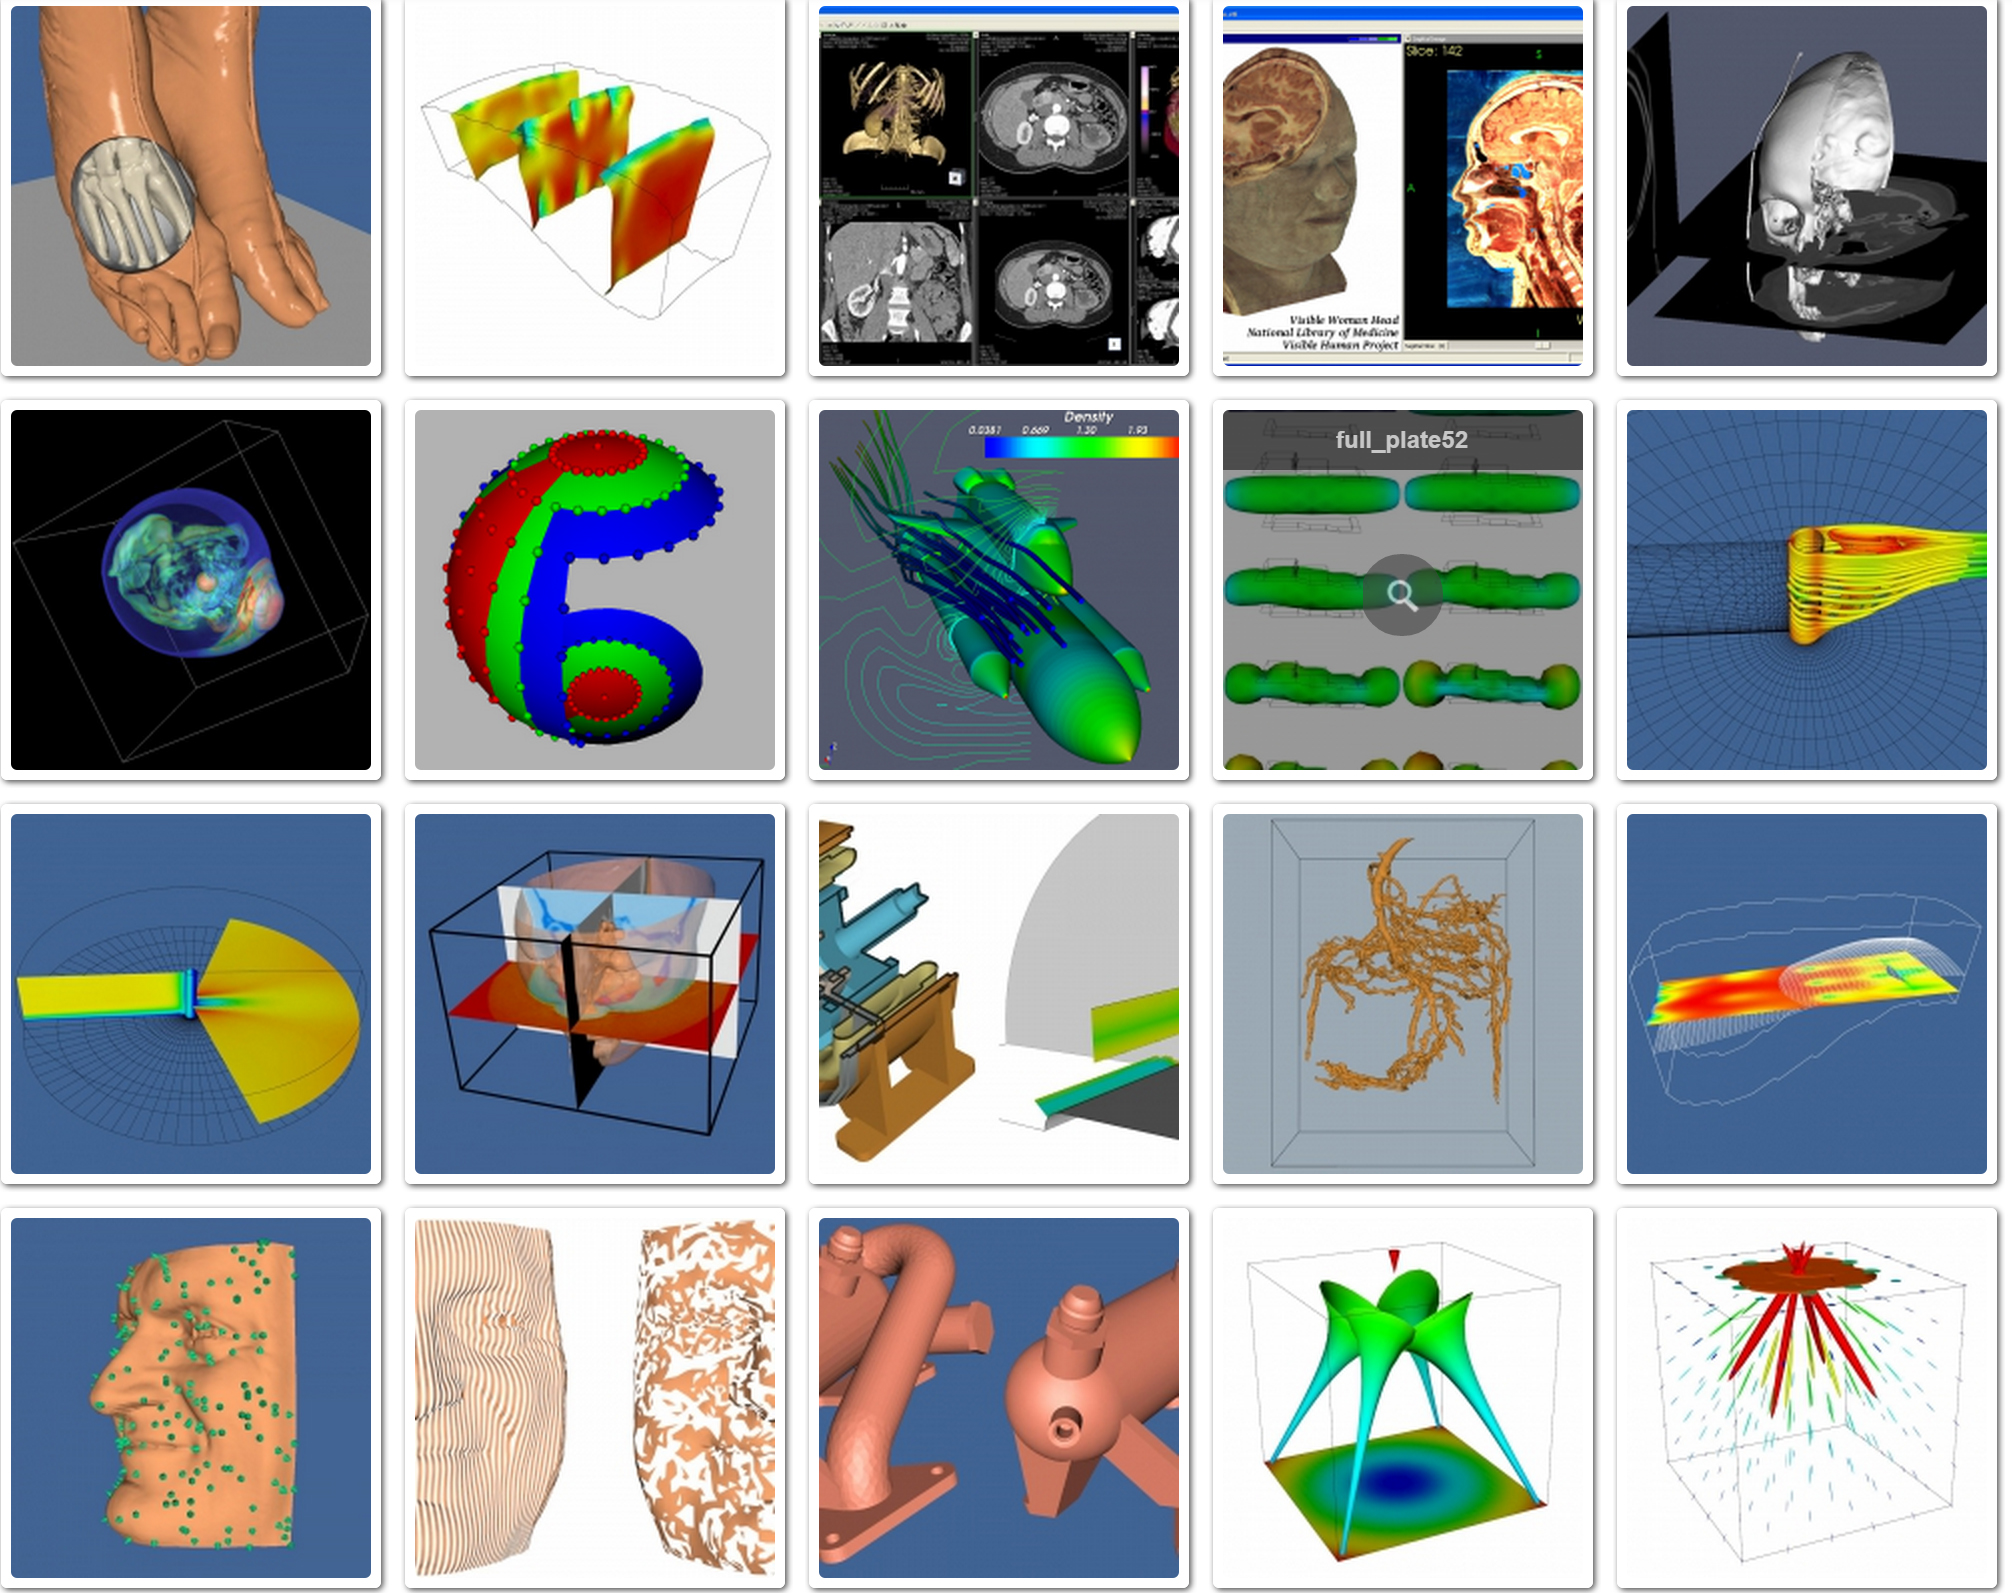
\includegraphics[width=0.9\linewidth]{graphics/vtk.jpg}
    \captionof{figure}[VTK Capabilities]{Different visualizations done with VTK.}
    \label{fig:vtkgallery}
\end{minipage}
Mayavi is probably one of the biggest, open source library for interactive 3D visualizations.
It is written 99.9\% in python, but relies on \ac{VTK} for rendering.
\ac{VTK} is one of the most advanced scientific visualization library, with a huge amount of visualization types. In figure \ref{fig:vtkgallery} you can see some of the visualization taken from the \ac{VTK} gallery\cite{VTKGallery}.

Mayavi shares some of its goals with Romeo, namely\cite{MayaviGoals}
\begin{itemize}
	\item An (optional) rich user interface with dialogs to interact with all data and objects in the visualization.
	\item A simple and clean scripting interface in Python, including one-liners, or an object-oriented programming interface. Mayavi integrates seamlessly with numpy and scipy for 3D plotting and can even be used in IPython interactively, similarly to Matplotlib.
	\item The power of the VTK toolkit, harnessed through these interfaces, without forcing you to learn it.
\end{itemize}
Obviously, the python part is not a shared goal, but creating an interactive 3D visualization library deeply embedded into a language is.
Mayavi together with VTK is a very big project and in this sense not really comparable to Romeo.
It amounts to a total of 3.642.105 lines of code written in 29 languages. The statistics can be found in table \ref{table:ParaviewStatistic} and \ref{table:VTKStatistic}.
The biggest difference is, that Romeo is implemented in a scientific programming language, while Mayavis core uses VTK which is mainly implemented in C++.
This has two big implications.
Firstly, if the language does not have native C++ compatible data types and an overhead less C++ interface, shipping a large stream of data to VTK becomes slow.
Secondly, one must know C++ to extend VTK. This makes it difficult to create customized visualizations.

In contrast, Romeo is implemented in one language, making these tasks very simple and efficient.


\subsubsection{Vispy}

Vispy is yet another interactive 3D visualization library. It is from the goals and development status the closest to Romeo.
These include\cite{VispyGoals}:

\begin{itemize}
	\item High-quality interactive scientific plots with millions of points.
	\item Direct visualization of real-time data.
	\item Fast interactive visualization of 3D models (meshes, volume rendering).
	\item OpenGL visualization demos.
	\item Scientific GUIs with fast, scalable visualization widgets (Qt or IPython notebook with WebGL).
\end{itemize}

It is a fairly new library, promising to use modern OpenGL and being able to achieve state of the art performance.
This is very similar to Romeo's goals, with the only difference being that Romeo is implented in Julia while Vispy is implemented in Python.
So the biggest differenciation between Romeo and Vispy will be found in the performance and the concrete feature set.


\pagebreak

\section{Requirements}

All building blocks in this thesis are developed with the purpose in mind to give the user the ability to visualize and interact with complex 2D and 3D data while being able to easily extend the library.
To enable this kind of functionality, a lot of parts of the infrastructure need to work seamlessly together.
Certain design choices had to be made to guarantee this. As speed is the most constraining factor, this chapter will start by introducing the design choices that had to be made in order to achieve state of the art speed.

\vspace{1em}
\begin{minipage}{\linewidth}
    \centering
    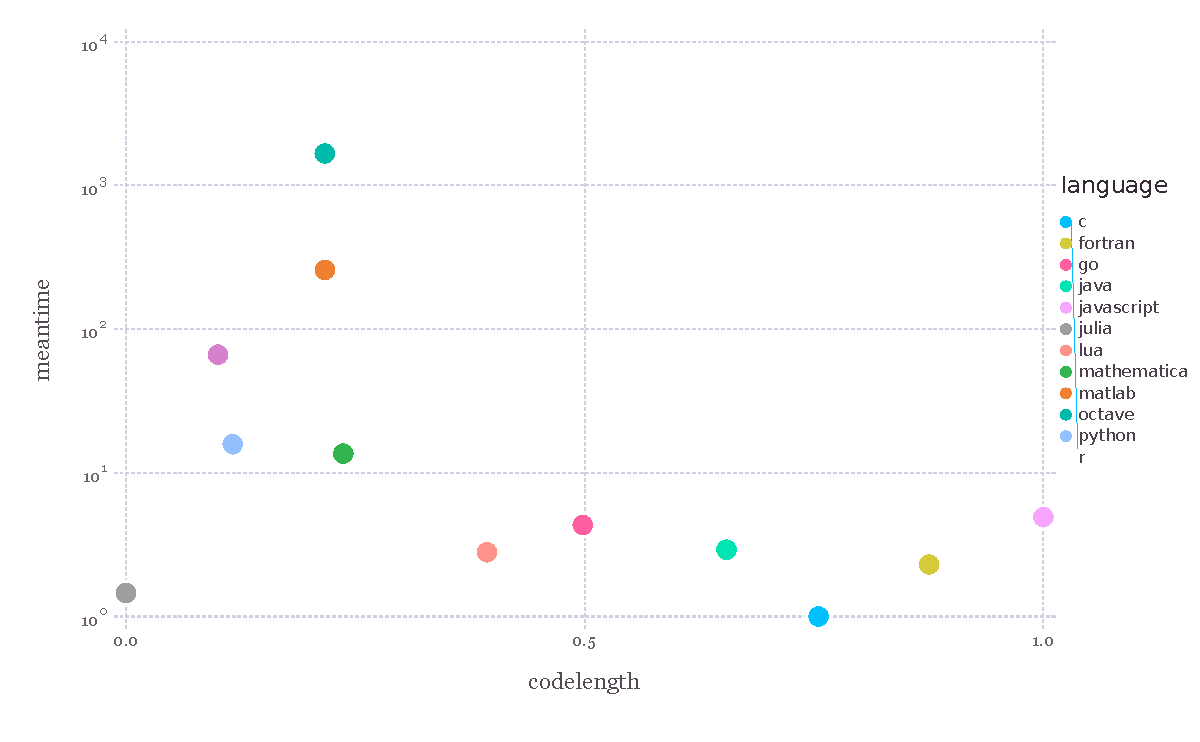
\includegraphics[width=0.9\linewidth]{graphics/julia_bench.pdf}
    \captionof{figure}[Volume Visualization]{Languages speed relative to C (averaged benchmark results), plotted against the length of the needed code (Source in Appendix).}
    \label{fig:juliabench}
\end{minipage}


\subsubsection{Speed}
Speed is mainly a usability factor. It is a factor, that can make a software unusable, or render it unproductive. Because of this, speed has taken a high priority in this thesis. 
As general coding productivity is also a concern, this thesis is set on using a high-level language.
Historically, these two demands can not be satisfied at the same time.
How to achieve state of the art speed with a high-level language is an ongoing research and basically the holy grail of language design. 
Julia promises to do exactly this, which is illustrated in figure \ref{fig:juliabench}. 
The code length is an ambiguous measure for conciseness, but if the code is similarly refactored and implements the same algorithm, it is a good indicator of how many lines of code are needed to achieve the same goal.
From this figure, we can conclude, that Julia at least comes close to its promises, which is why it has been chosen as the programming language.

There are a lot of libraries out there which can be used as a basis for implementing a 3D visualization library.
If you start to take the previous demands into account, the options shrink down considerably.
The visualization library should be implemented in one high-level language, which can be used for scientific computing and has state of the art speed. 
At this point, there are close to zero libraries left. As you can see in figure \ref{fig:juliabench}, Matlab, Python, and R disqualify, as they are too slow. JavaScript, Java, Go, and Lua are missing a scientific background and the others are too low level for the described goals.
This leaves only Julia, but in Julia there were no 3D libraries available, which means that one has to start from scratch.
There are only a couple of GPU accelerated low-level libraries available, namely Khronos's \ac{OpenGL}, Microsoft's DirectX, Apple's Metal and AMD's Mantel, which are offering essentially the same functionality. 
As only \ac{OpenGL} is truly cross-platform, this leaves \ac{OpenGL} as an option.
To access \ac{OpenGL} from within Julia a wrapper had to be written. 
This leaves us with one binary dependency not written in Julia, namely the video driver, which implements \ac{OpenGL}.

Measurement of success is pretty straightforward, but the devil is in the detail.
It is easy to benchmark the code, but quite difficult to find a baseline, as one either has to implement the whole software with an alternative technology or one has to find similar software.
This thesis will follow a hybrid strategy, comparing some simple implementations with different technologies and choose some rivaling state of the art libraries as a baseline.

\subsubsection{Extensibility}
Extensibility is an important factor in scientific computing, as a lot of flexibility is needed when exploring new horizons. 
It is not only that, but also a great factor determining the growth of a library. The more extensible the software is, the higher is the probability that someone else contributes to it.
In order to write extensible software, we first have to clarify what extensibility is.
Extensible foremost needs that the code is accessible. There are different levels of accessibility. 
The lowest level is closed source, where people purposely make the code inaccessible. While this is obvious, it is just a special case of not understanding the underlying language. 
Shipping binaries without open sourcing the code means that the source is only accessible in a language which is extremely hard to understand, namely the machine code of the binary. So another example for inaccessibility is to write in a language that is difficult to understand. 
Other barriers are obfuscated language constructs, difficult compilation procedures, missing documentation and cryptic highly optimized code.
Furthermore, the design of the library in the whole is an important factor for extensibility. It is not only important, that all parts are understandable, but also, that every independent unit in the code solves only one problem. 
This guarantees that one can quickly exchange it, or use it somewhere else where the same problem needs to be solved.
If this is guaranteed, re-usability in different contexts becomes much simpler. 
This allows for a broader user base, which in turn results in higher contributions and bug reports.
Short concise code is also important, as it will take considerably less time to rewrite something, as the amount of code that has to be touched is shorter and less time is spent on understanding and rewriting the code.

So the code written for this thesis will be open source, modular, written in a high-level language and concise.

This is pretty difficult to measure as these are either binary choices, which are followed or not or higher level concepts like writing concise code, which can be a matter of taste.
To get an idea of the effectiveness of the strategy, usage patterns and feedback from Github will be analyzed.

\subsubsection{Event System}
The event system is a crucial part of the library, as the proclaimed goal is to visualize dynamic, animated data.
This means, there are hard demands for usability and speed on the event system.
The chosen event system has an immediate influence on how to handle animations. 
The cleanest abstraction for animations and events are signals. Signals represent values that change over time.
If well implemented, it makes it natural to reason about time, without the need of managing unrelated structures and callback code.

\subsubsection{Interfaces}

Working with a computer means working with interfaces to a computer, which in the end simply juggles around with zeros and ones. There is a huge hierarchy of abstractions involved, to make this process of binary juggling manageable to the human.
We already dealt with the lowest relevant abstraction, which was the choice of programming language.
The next level of abstraction is the general architecture of the modules, which has been discussed previously. 
This chapter is about the API design choices that have been made.

The first \ac{API} is the \ac{OpenGL} layer. 
The chosen philosophy was to make the wrapper for native libraries as thin and reusable as possible and a one-to-one mapping of the underlying C-library.
This guarantees reusability for others, who want to work with the low-level library. Also, they might disagree with some higher-level abstractions and prefer to write their own.

Over this sits an abstraction layer needed to simplify the work with \ac{OpenGL}.
With this abstraction, the actual visualization library is implemented.

\ac{API}s for visualization libraries are very difficult to realize, as there are endless ways of visualizing the same data.
The design choice here was to use Julia's rich type system to better describe the data. 
Julia makes this possible, as you can create different types for the same data without loosing performance.
So you can have a unit like meters represented as a native floating point type and have the visualization specialize to this.
Like this you can have a single function, e.g. \textit{visualize}, that does create a default visualization for different data types. 
Instead of manually passing additional information to the visualization function all information is coded into the type itself.
Together with the event system which consists of signals, it is possible to edit and visualize rich data over a simple interface. This is perfect for visual debugging, as it is always the same function call applied to the data. 
With this, variables can be visualized without further user interaction.
Default visualizations can be created like this, but for a more fine grained control of the visualization this will not suffice.

To pass addition information, key word arguments are used together with a style type, which control the chosen defaults and the visualization.
So for a float matrix, the default visualization may be a height-field, but passing the style \texttt{text} to the function might change the default to render a textual representation of the matrix.
This makes it easy to extend the visualize function, as the user just has to overload the function with a custom style together with optional key word arguments.
Finally, there are also graphical user interfaces developed for this thesis. As also optimizing them is out of the scope of this thesis, they are kept very simple.
The measurement of success is again relatively difficult to achieve.
Best would be to make a user poll to get actual feedback from people that use the software. This is a pretty demanding task, so instead the interface will just be evaluated analytically.


\section{Used Technologies}

\subsection{The Julia Programming Language}

The basic introduction of Julia has already been given in the Background chapter.
This chapter is focused on how to write programs with Julia and if it satisfies the requirements.
Most influential language construct are its hierarchical type system and multiple dispatch.
Multiple dispatch is in its core function overloading at runtime. 
To better understand multiple dispatch, one has to be familiar with Julia's type system.
The type system builds upon four basic types. 
Composite types, which are comparable to C-Structs, parametric composite types, bits types, abstract and parametric abstract types.
While the first three are all concrete types, abstract types can not be instantiated but are used to build a type hierarchy.
Every concrete type can only inherit from one abstract type, while abstract types can also inherit from abstract types.
Bit types are just immutable, stack allocated memory chunks, usable for implementing numbers.
You can build type hierarchies like this:
\begin{lstlisting}
abstract Number
abstract FloatingPoint{Size} <: Number # inherit from Number
bitstype 32 Float32 <: FloatingPoint{32} # inherit from a parametric abstract type
type Complex{T} <: Number
    real::T
    img::T
end
\end{lstlisting}

With this type hierarchy you can overload functions with abstract, concrete or untyped arguments.

\begin{lstlisting}
foo{T}(y::Complex{T}, y::Float32) = println("some number: ", x, " some complex Number: ", y) # shorthand function definition
function foo(x)
    println("overloading foo with a new unspecific signature")
end
\end{lstlisting}

What will happen at runtime is, that Julia compiles a method specialized on the arguments which result in overloading the function with a method with the concretely typed arguments.

In the case of \textit{foo}, it is initially overloaded with two methods.
Now, if you call \textit{foo} with one \textit{Float32} argument, a new method will be added at run time specialized to the\textit{Float32} argument.
Like this, if the function does not access non constant global values, all types inside the function will be known at call time.
This allows Julia to statically compile the function body, while propagating the type information down the call tree.

With multiple dispatch, Julia is a functional oriented language. But there are also ways to give Julia a more object oriented feel.
Functions are first-class, so they are easy to pass around. 
They can be bound to variables and can then be called like normal functions via the variable name. This implies that functions can also be bound to objects.
There is no self-reference available in Julia so the object still needs to be passed to the function via the arguments

Another of the most crucial features is the very simple, overhead less C-Interface. 
Thanks to the binary compatibility of \ac{LLVM}'s emitted assembly, a C function call to a shared library inside Julia has the same overhead as it would be from inside C\cite{CCALL}. 
This is perfect for integrating low-level libraries like \ac{OpenGL} and \ac{OpenCL}.

Julia's performance is crucial for this thesis. 
If Julia does not perform close to C it would weaken the whole argument of writing the visualization library in Julia.
This is why a performance analysis is done to prove that Julia is a good choice for a high performance visualization library.

It is a very tedious task to write representative benchmarks for a programming language. 
The only way out is to rely on a multitude of sources and try to find analytical arguments.
In this thesis, Julia's own benchmark suite will be used in addition to some real world benchmarks.
In addition, the general compiler structure of Julia will be analyzed to find indicators for the limits of Julia's performance.

\vspace{1em}
\begin{minipage}{\linewidth}
    \centering
    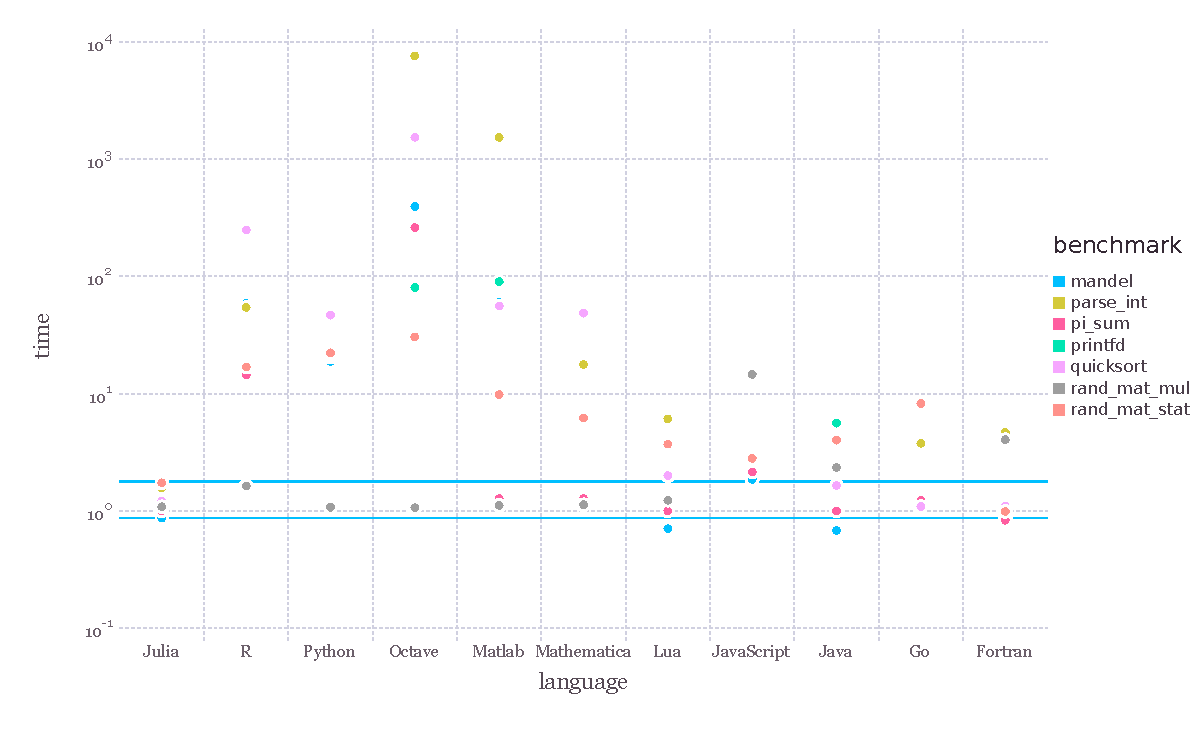
\includegraphics[width=0.9\linewidth]{graphics/juliabench.pdf}
    \captionof{figure}[Julia Performance]{Julia's performance compared to other languages, taken from Julia's micro bench suite \cite{JuliaBench}. Smaller is better, C performance = 1.0.}
    \label{fig:juliabench}
\end{minipage}

In the first benchmark from figure \ref{fig:juliabench}, we can see that Julia stays well within the range of C Speed. 
Actually, it even comes second to C-speed with no other language being that close.
This is a very promising first look at Julia, but it should be noted, that these benchmarks are written by the Julia core team and the performance of a language is a moving target.
So it is not guaranteed, that there is no bias favoring Julia in these benchmarks.
Another benchmark was found, which compares C++, Julia and F\#. It was created by Palladium Consulting which should not have any interest in favoring any of the languages.
They compare the performance of C++, Julia and F\# for an IBM/370 floating point to IEEE floating point conversion algorithm.
The results\cite{JuliaFSCpp} have been, that F\# comes out last with 748.275 ms, than Julia with 483.769 ms and finally C++ with 463.474 ms. 
At the citation time, the Author had updated the C++ version to achieve 388.668 ms. 
It looks like the author was only working on making the C++ version faster, so it can not be said that the other versions could not have been made faster too.

The last Julia benchmark is more real world oriented. 
It is comparing Finite Element solver, which is an often used algorithm in material research and therefore represents a relevant use case for Julia.

\begin{table}[htbp]
    \centering
    \begin{tabular}{l|c|c|c}
        \hline
        \textbf{N}  & \textbf{Julia} & \textbf{FEniCS(Python + C++)}  & \textbf{FreeFem++(C++)}\\
        \hline
        121         & 0.99           & 0.67             & 0.01 \\
        2601        & 1.07           & 0.76             & 0.05 \\
        10201       & 1.37           & 1.00             & 0.23 \\
        40401       & 2.63           & 2.09             & 1.05 \\
        123201      & 6.29           & 5.88             & 4.03 \\
        251001      & 12.28          & 12.16            & 9.09 \\
        \hline
    \end{tabular}
    \captionof{table}[FEM Benchmark]{Performance of a FEM solver written in Julia compared to some existing libraries. \cite{FMSolver}}
    \label{table:fembench}
\end{table}
These are remarkable results, considering that the author states it was not a big effort to achieve this. After all, the other libraries are established FEM solvers written in C++, which should not be easy to compete with.

This list could go on, but it is more constructive to find out Julia's limits analytically.
As already mentioned, Julia is statically compiled at runtime. This means, as long as all types can be inferred at runtime, Julia will have in the most cases identical performance to C++.
The biggest remaining difference in this case is the garbage collection. Julia 0.3 has a mark and sweep garbage collector, while Julia 0.4 has an incremental garbage collector.
As seen in the benchmarks, it does not necessarily introduce big slowdowns.
But there are issues, where garbage collection introduces a significant slow down\cite{ReadDlmGC}.
Analyzing this further is not in the scope of this thesis, though. 
But it can be said that Julia's garbage collector is very young and only the future will show how big the actual differences will be.
Another big difference is the difference in between different compiler technologies.
Julia uses \ac{LLVM} for compilation.
In order to further understand Julia's potential, a further look at LLVM is taken in the next section.

\subsubsection{\ac{LLVM}}

\ac{LLVM} is a compiler infrastructure, which has front ends for different languages and compiles to different platforms like x86, ARM, \ac{OpenCL} (SPIR) and \ac{CUDA} (NVPTX). 
A language designer must create an \ac{AST} which \ac{LLVM} can convert into \ac{LLVM} \ac{IR}. This \ac{IR} forms a standardized basis for any optimization step. Every language that can be converted to \ac{LLVM} \ac{IR} can be combined at this level.\ac{LLVM} offers many optimizations, but also third party optimization steps can be integrated.
This yields superior language interfacing, as inlining and other optimizations can be done over the boundary of one language.

\ac{LLVM}'s concept is effective, as you can accumulate state of the art optimizations in one place, making them accessible to many languages. Because of the many back-ends, languages that use \ac{LLVM} can run on many architectures. While Julia does not support all back-ends yet, support will be added in the future. 
\ac{LLVM} is also used by Clang, the C/C++ front end for \ac{LLVM} rivaling \ac{gcc} and it is used by Apple's programming language Swift and for Mozilla's language Rust.
This makes \ac{LLVM} a solid basis for a programming language, as these are highly successful projects guaranteeing \ac{LLVM} further prospering.
To see where \ac{LLVM} stands considering performance, one can compare it with \ac{gcc}, which is one of the most successful open source compilers for C++.
If C++ code that is compiled with \ac{gcc} is much faster than the same code compiled with \ac{LLVM}, the \ac{gcc} version will also be faster as a comparable Julia program.
In order to investigate the impact of this, a benchmark series written by Phoronix will be analyzed.
They benchmarked \ac{gcc} 4.92 against \ac{LLVM} 3.5 and \ac{LLVM} 3.5 against \ac{LLVM} 3.6.
Here is a summary of their exhaustive benchmarks:
\begin{table}[ht]
  \centering
  \begin{tabular}{l|c|c}
    \hline
    \textbf{Statistic} & \textbf{\ac{gcc} vs \ac{LLVM} 3.5} & \textbf{\ac{LLVM} 3.5 vs \ac{LLVM} 3.6} \\
    \hline
    mean & 0.99 & 0.99 \\
    median & 0.97 & 1.00 \\
    maximum & 1.48 & 1.10 \\
    minimum & 0.39 & 0.88 \\
    \hline
  \end{tabular}
    \captionof{table}[gcc vs llvm summary]{Summary of the Phoronix benchmark. Unit is speedup of \ac{LLVM}, bigger is better. \cite{LLVM35vsLLVM36}\cite{LLVMvsGCC}\cite{Phoronix}}
    \label{table:gccvsllvm}
\end{table}

The full tables can be found in the appendix under the table \ref{table:llvm35vsllvm36} and \ref{table:llvmvsgcc}.
The results suggest, that \ac{LLVM} is well in the range of \ac{gcc}, even though that there can be big differences between the two.
These are promising results, especially if you consider that \ac{LLVM} is much younger than \ac{gcc}. 
With big companies like Apple\cite{GoogleAppleLLVM}, Google\cite{GoogleAppleLLVM}, Mozilla\cite{Rust}, AMD\cite{LLVMAMD}, NVidia\cite{LLVMNvidia} and Microsoft\cite{MicrosoftLLVM} being invested in LLVM, it is to be expected that \ac{LLVM} will stay competitive, which means Julia should in theory stay competitive as well.


\subsection{\ac{OpenGL}}

\vspace{1em}
\begin{minipage}{\linewidth}
    \centering
    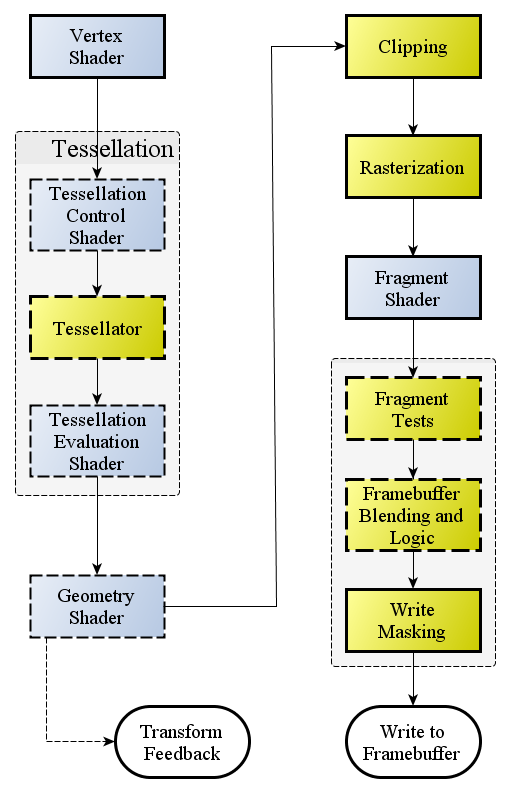
\includegraphics[width=0.5\linewidth]{graphics/RenderingPipeline.png}
    \captionof{figure}[OpenGL]{Diagram of the Rendering Pipeline. The blue boxes are programmable shader stages. Arrows show the flow of data\cite{OpenGLPipeline}}
    \label{fig:opengl}
\end{minipage}


\ac{OpenGL} is a low-level graphics API implemented by the video card vendor via the video driver. 
As such it does not offer much abstraction over the actual \ac{GPU}, but instead offers high flexibility and performance.
\ac{OpenGL} 1.0 was released in 1992 and the current version is 4.5.
A critical element when developing \ac{OpenGL} applications is, that not all video drivers implement the newest \ac{OpenGL} standards.
As a result, one has to decide which \ac{OpenGL} version to target, trading between modernity and platform support.
For Romeo, it was decided to support \ac{OpenGL} 3.3 as the lowest bound, as it is sufficiently available, while still having most of the modern features.
All features that help to call less OpenGL functions can be considered as modern, as they take away the load from the CPU.
The modern features used in this thesis include instance rendering, vertex arrays and \ac{GLSL} shader.

In figure \ref{fig:opengl} you can see the basic architecture of an OpenGL program pipeline.
As the description states, the blue boxes are programmable shaders, while the dotted boxes are optional parts of the pipeline.
The yellow boxes describe stages which are not directly accessible. They are part of the global OpenGL state, which can be set via OpenGL commands.

So in order to have a working OpenGL rendering pipeline one needs to write at least a vertex shader and a fragment shader.
All shaders are compiled and linked into a program object, which can be executed on the \ac{GPU}.
Shaders are written in a C dialect specialized for vector operations.
You feed shaders with data via buffers, textures and uniforms. Buffers are 1D arrays, textures 1D/2D/3D arrays with both having their own memory, while uniforms live in the program object.

The different shaders are usually used to apply geometric and perspective transformations and calculating the light.
In newer APIs general compute operations are available, making it possible to create more flexible shader stages.
Displaying objects can only be achieved by rasterizing pixels to the frame buffer via the fragment shader.
The frame buffer can be sent directly to the monitor.
Frame buffers can contain multiple render targets, which are the buffers the fragment shader can write to.
The write operation is heavily restricted. The fragment shader can only write to the location calculated by the vertex shader and simultaneously reads from the frame-buffer are not possible. 
This restriction exists to allow for the massive parallel execution model that OpenGL uses to speed up rendering times.

The usual set of render targets includes a depth channel, stencil buffer and of course the color buffer.
The depth channel is usually used to discard all fragments that are behind another fragment (known as depth test), while the stencil buffer can be used to discard arbitrary fragments based on the stencil mask. 
Custom render targets can be created in newer OpenGL versions which can be directly addressed via the fragment shader.
Here is a simple minimal example for a program rendering some vertex data with a flat color to the screen.

\begin{lstlisting}
//Vertex Shader
in vec3 vertex; // vertex fed into the shader via a buffer
uniform mat4 projection; // Projection matrix
uniform mat4 view; // View matrix, setting rotation and translation of the camera
void main()
{
    gl_position = projection*view*vec4(vertex, 1); // apply transformations to vertex and output to fragment shader
}
//Fragment shader
out vec4 framebuffer_color; //color render target, which will get written into the display framebuffer
void main()
{
    framebuffer_color = vec4(1,0,0,1); // write a red pixel at gl_position from the vertex shader.
}
\end{lstlisting}

All visualization code is written in OpenGL shaders, which are compiled and executed via GLAbstraction.

\subsection{Reactive}
Reactive\cite{Reactive} is a functional event system designed for event driven programming.
It implements Elm's\cite{Elm} signal based event system in Julia.
Signals can be transformed via arbitrary functions which in turn create a new signal.
This simple principle leads too a surprisingly simple yet effective way of programming event based applications.

\begin{lstlisting}
a = Input(40)       # an integer signal.
b = Input(2)        # an integer signal.
c = lift(+, a,b)    # creates a new signal with the callback plus. Equal to c = a+b
lift(println, c)    # executes println, every time that c is updated. 
push!(a, 20)        # updates a, resulting in c being 22
#prints: 22
push!(b, 5)         # updates a, resulting in c being 22
#prints: 25
\end{lstlisting}

Lifting a signal creates a callback, which gets called whenever the signal changes.
There are more operations than lifting, like folding, merging, filtering and so on.
With this, one can build up a complex tree of operators which will get applied to the origin signal.
For the concrete case of Reactive, every signal carries around a list of children and parents.
Each signal has a rank, in order to build up a sorted heap with these information.
So every time a signal is updated, the heap can be traversed and the functions get applied in the right order, updating all the values of the children.
Reactive is used in all parts of the library. It builds the basis for the camera code, the widgets and any value that needs to be animated is realized via a signal.

\subsection{GLFW}
GLFW\cite{GLFW} is a cross platform \ac{OpenGL} context and window creation library written in C.
GLFW allows to register callbacks for a multitude of events like keyboard, mouse and window events.
Every operating system exposes this functionality in a slightly different way, making it very hard to create a window and to retrieve window events.
So a library like GLFW is crucial if one does not want to waste a lot of time just to implement all the corner cases for all the different operating systems out there.
In addition, GLFW exposes low level features like the operating systems context handle.
This can be used for creating advanced contexts that share memory with another context.
Romeo does not use this feature yet, but it makes GLFW a future proof choice.


\section{Implementation}

\vspace{1em}
\begin{minipage}{\linewidth}
    \centering
    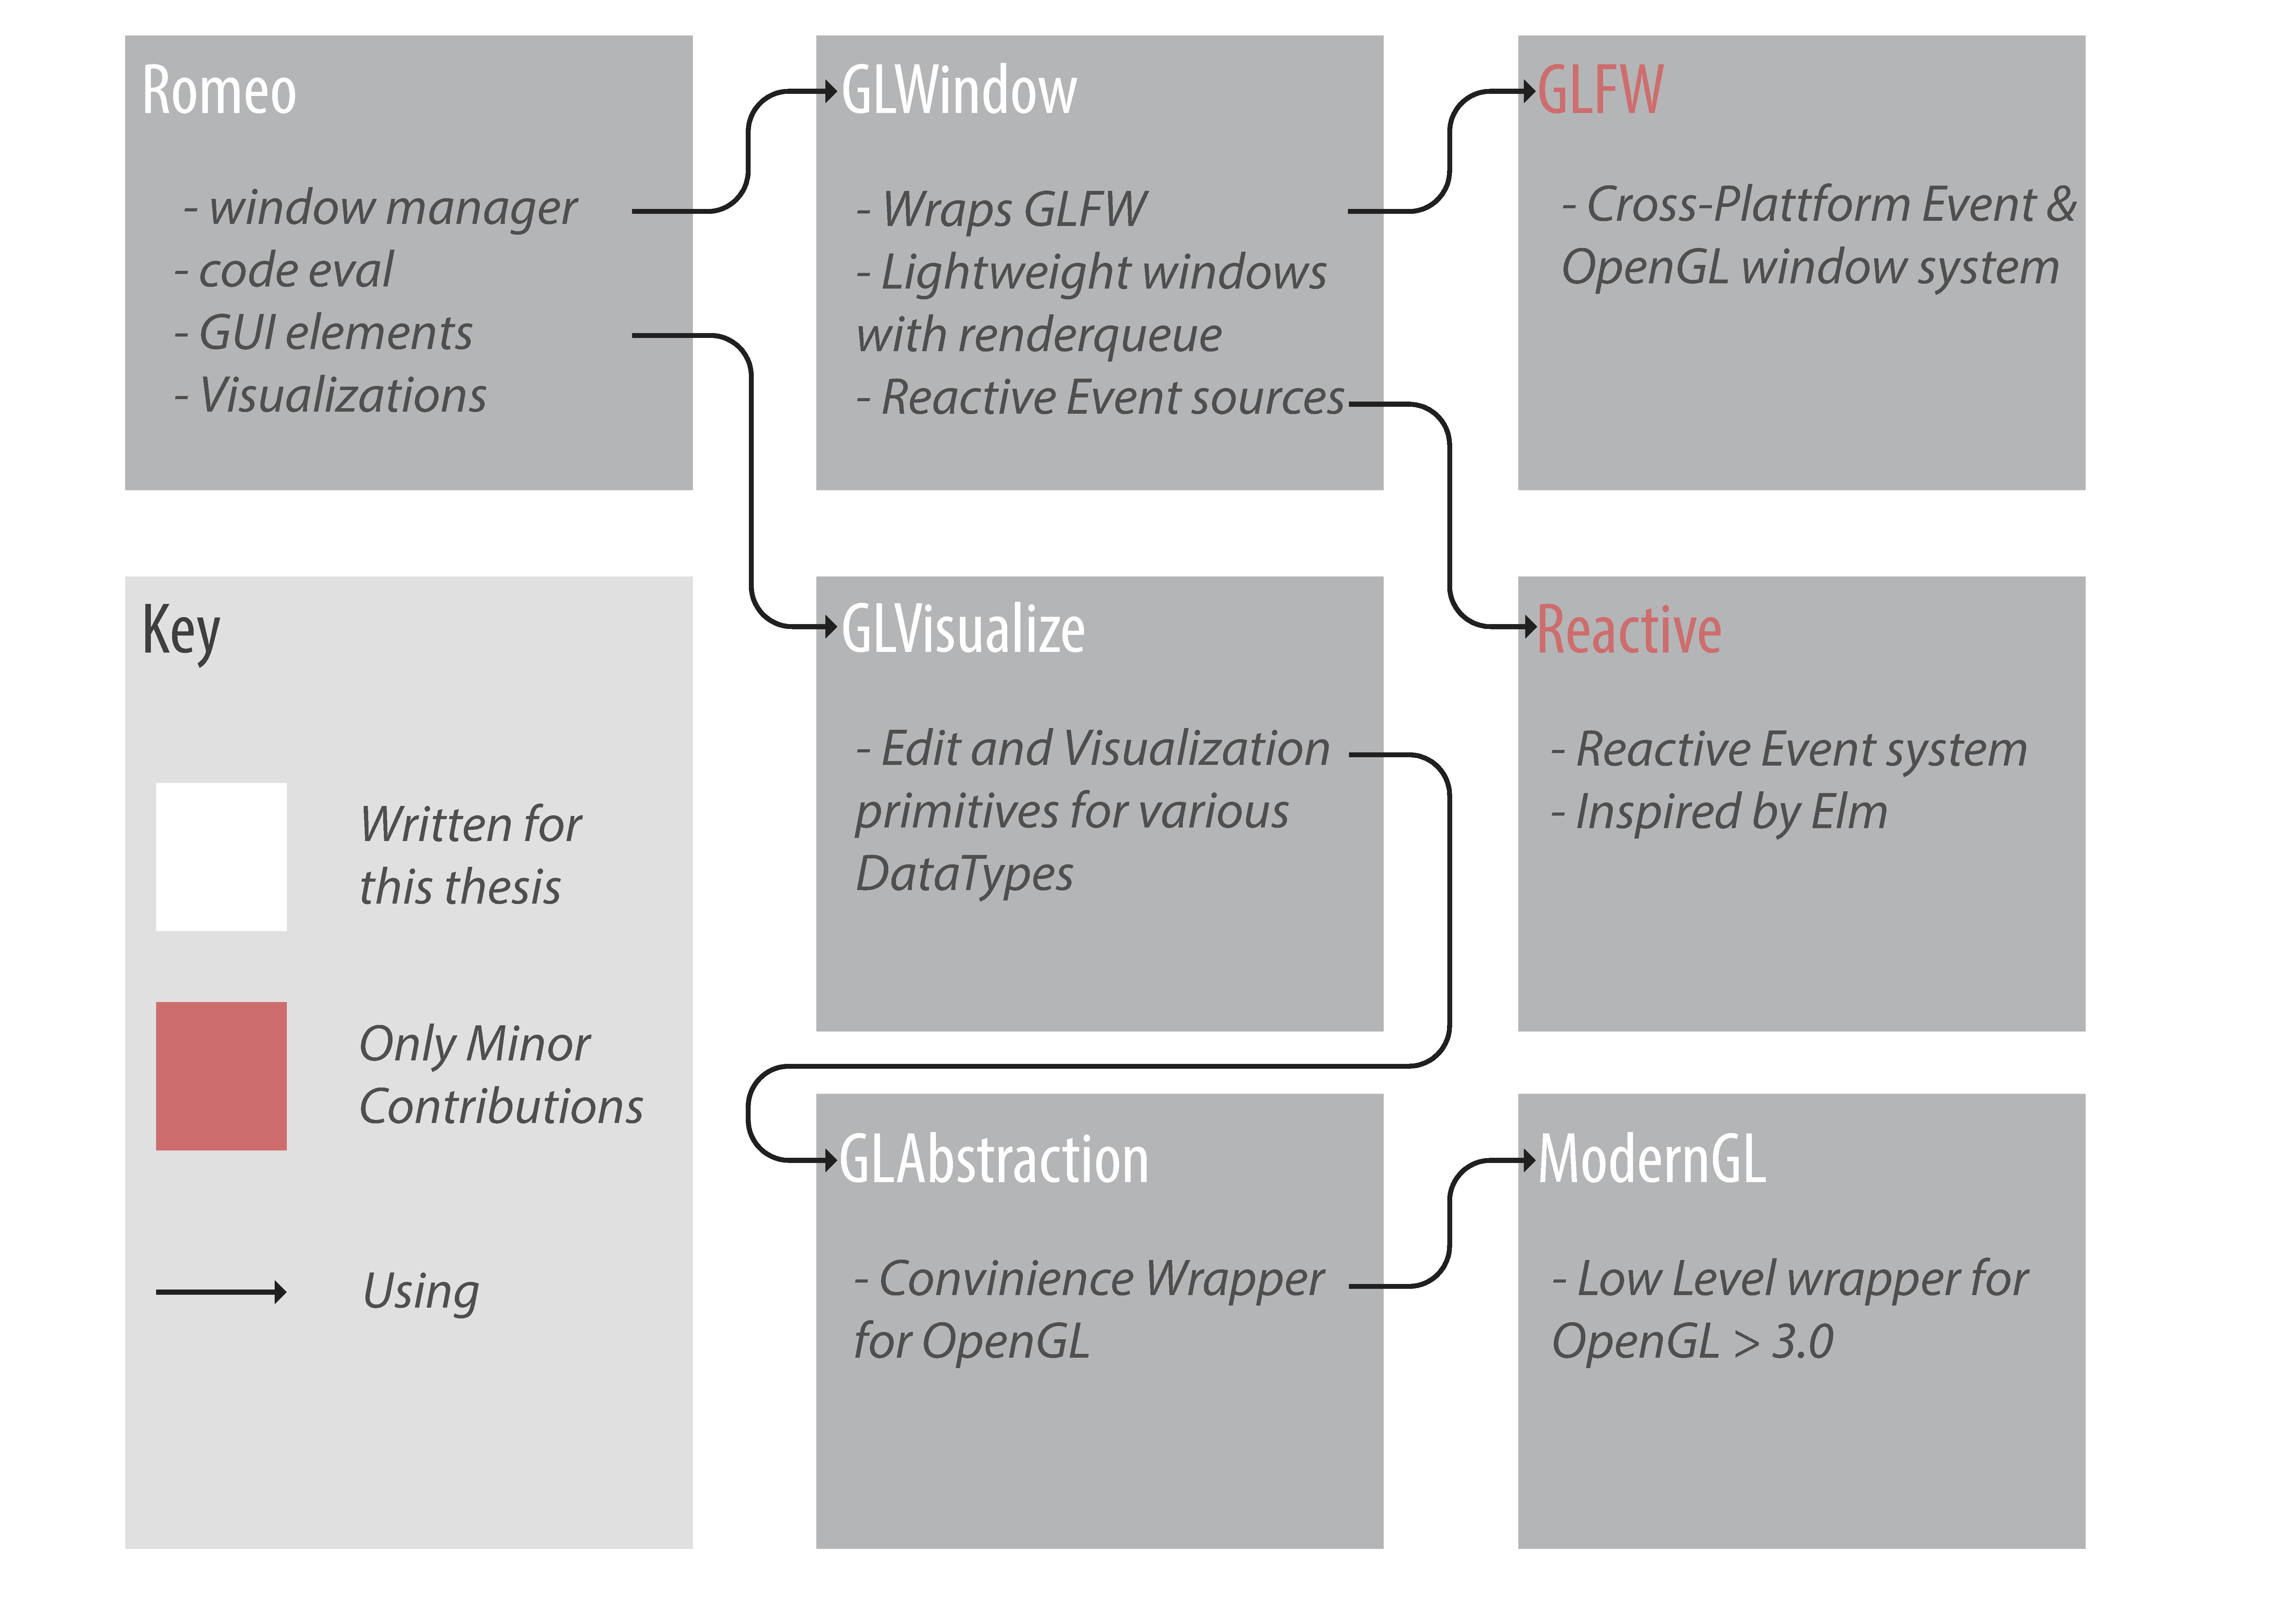
\includegraphics[width=0.9\linewidth]{graphics/architecture.pdf}
    \captionof{figure}[Architecture]{Main modules used in Romeo and their relation (simplified).}
    \label{fig:architecture} 
\end{minipage}


This chapter is about the implementation of Romeo.
The Romeo package itself is small and just defines the high-level functionality of the editor.
This includes window layout and connecting all the different event sources to create the wanted behavior.
To do this, Romeo relies on a multitude of packages, which step for step abstract away the underlying low-level code that is used to do the window creation and rendering. 
Like already pointed out in the requirements, special care has been taken to make all modules self sufficient. 
Every single package can be used for other applications, which allows for higher flexibility and a broader user base.
ModernGL can be used by any OpenGL project which strives to build a low-level OpenGL program.
GLWindow and GLAbstraction can be used to build slightly higher level OpenGL visualizations. 
GLVisualize can be used to build other interactive visualization packages besides Romeo.

As you can see in figure \ref{fig:architecture}, Romeo uses GLVisualize for creating \ac{GUI} elements and the visualizations. Romeo's code evaluation is done via Julia build-in functions and text fields are displayed with GLVisualize.
Windows are managed with GLWindow. 
GLWindow creates an OpenGL window with the help of GLFW and converts all window events into Reactive's signals. 
It also offers a very simple render queue, for rendering graphics attached to a window.
Signals are not only used as the event sources, but are also the main abstraction for time varying values in GLVisualize.
GLVisualize is the main package offering the rendering functionality and the editor widgets like text fields and sliders.
For rendering GLVisualize relies on GLAbstraction, which defines a high-level interface for ModernGL.
ModernGL does the \ac{OpenGL} function loading and exposes all the function and Enums definitions from \ac{OpenGL} with version higher than 3.0.



\subsection{ModernGL}
\ac{OpenGL} is implemented by the video card vendor and is shipped via the video driver, which comes in the form of a C library.
The challenge is to load the function pointers system and vendor independent. 
Also one further complication is, that depending on the platform, 
function pointer are only available after an \ac{OpenGL} context was created and may only be valid for this context. \cite{wgl}
This problem is solved by initializing a function pointer cache with null and as soon as the function is called the first time the real pointer gets loaded.

The OpenGL function loader from ModernGL has undergone some changes over the time.
Starting with a very simple solution, there have been pull requests to improve it.
The current approach in ModernGL master was not written by myself, but by the Github user aaalexandrov.
Before aaalexandrov’s approach, the fastest approach would have used a pretty new Julia feature, named staged functions.
It should in principle yield the best performance as it compiles a specialized version of the function when it gets called for the first time. This is perfect for \ac{OpenGL} function loading. When the staged function gets called the pointer can be queried and gets inlined into the just in time compiled function.

Staged functions only work with the newest Julia build, which is why aaalexandrov’s approach was favored.


\subsection{GLAbstraction}
GLAbstraction is the abstraction layer over ModernGL.
It wraps \ac{OpenGL} primitives like Buffers and Textures in Julia objects and hooks them up to Julia's garbage collector. It also makes it easy to create them from Julia data types like arrays and images.
Additionally, it implements convenient functions to load shader code and it makes it easy to feed the shader with the correct data types.
Besides supplying an abstraction layer over \ac{OpenGL}, it also offers the linear algebra needed for the various 3D transformation and camera code.
Building upon that, it defines a signal based perspective and orthographic camera type.

Signals are an important part of the infrastructure not only for the camera, but for everything that changes.
As an example, the function that creates a program also takes signals of shader source code. 
With every source code update the OpenGL program gets recompiled, making it possible to interactively develop OpenGL shader. The signal can come from file updates, or from some text editing widget inside Julia.

One of the main data types is the \textit{RenderObject}.
It combines uniforms, OpenGL buffers and textures and OpenGL programs. One can call \textit{render(::RenderObject)}, which executes the program with the given uniforms and buffers loaded into the program. 
Like this, making visualizations with GLAbstraction turns into writing the shader and then combining it with the needed data in form of OpenGL types.
When the program includes a fragment stage, this means calling \textit{render} results in the object being displayed on the screen. But its also possible to use compute shaders with \textit{RenderObjects}, which then just writes into the supplied buffers without displaying anything.

A lot of OpenGL functions are bothersome to use from inside Julia, as the output has to be pre-allocated and gets then passed to the function.
These functions have been overloaded in GLAbstraction to return the value.
So with only ModernGL the code would look like this:
\begin{lstlisting}
result = Ref{GLint}(-1) #using Julia's reference type
glGetShaderiv(shaderID, GL_COMPILE_STATUS, result)
result = result[] # dereferencing
\end{lstlisting}
With GLAbstraction this becomes possible:
\begin{lstlisting}
result = glGetShaderiv(shaderID, GL_COMPILE_STATUS)
\end{lstlisting}

Similarly, OpenGL does not overload functions, which means function that do the same for different types have a base name with different suffixes to indicate the type.
The function with the most methods is \textit{glUniform}, which has 34 functions for all the different uniform types. With GLAbstraction, \textit{glUniform} has been overloaded for all different types, including arrays and signals. So one can simply call \textit{glUniform} on the type without the need of looking up the correct suffix.
This has been achieved with a combination of simple overloading and staged functions. The staged function puts together the right function name and inlines it into the \textit{glUniform} method specialized to the argument type.

A lot more of these simplifications have been done in order to leverage the usage of OpenGL inside Julia.

\subsection{GLWindow}
GLWindow is a lightweight wrapper around GLFW.
It mainly offers a screen type, which contains signals for all the different GLFW events. 
It also offers a hierarchical structure for nesting screens.
All the screen areas are signals, which makes it easy to change the screen area. 
This makes it simple to implement windows that react to changing the size of the windows or resized objects.

\subsection{Event System}

The event system was challenging to integrate for several reasons.
First of all Reactive is a functional event system, while \ac{OpenGL} relies heavily on global states, which are two perpendicular concepts.
Also, it does not allow to rearrange the event tree. 
In other words, you can not create sub trees in advance and then fuse them together at run time.
This has lead to the design choice, that the signals are sampled from a render loop.
This is sub-optimal, as sampling artifacts can occur, and frames are rendered even if the scene does not change.
In the future it will be desirable to work around this and bring the elegant functional approach from Reactive to OpenGL.


\subsection{GLVisualize}

\vspace{1em}
\begin{minipage}{\linewidth}
    \centering
    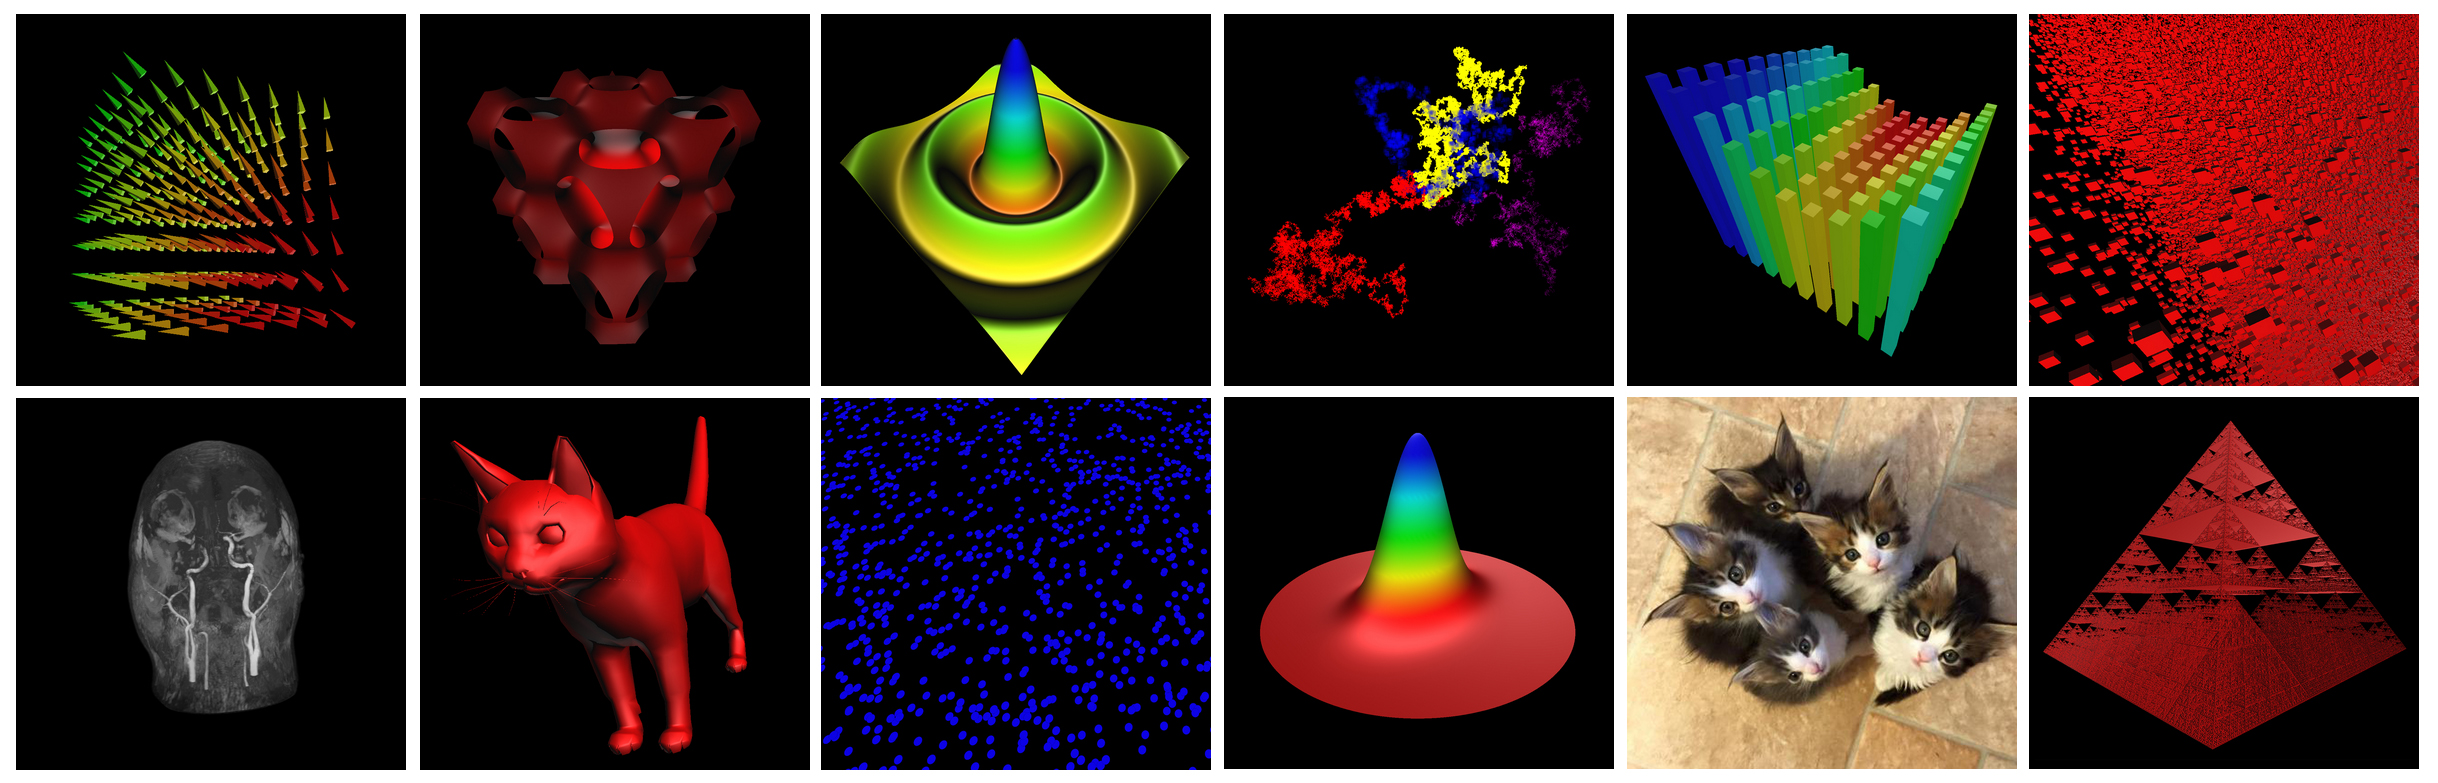
\includegraphics[width=0.9\linewidth]{graphics/glvisualize.jpg}
    \captionof{figure}[Visualisations]{Different visualizations rendered with GLVisualize.}
    \label{fig:glvisualize}
\end{minipage}

GLVisualize implements the main functionality of this library.
Its structure is quite simple. 
It relies as much as it can on common Julia data types and creates specialized visualizations for them via dispatch.
So instead of offering differently named functions for different visualizations, there is just one function with lots of methods for different types.
This has two advantages.
First, it makes it very easy to use for visual debugging, as any value can be displayed immediately without any user interaction.
Secondly, the user does not have to remember or lookup the function name, as long as there is a default visualization for the type he is working with.
The next design goal was to make this fit for dynamic data, which resulted in relying on as little transformation of the data as possible and directly transferring it to the GPU.
Depending on the complexity of the visualization, this means the visualization can be updated with as little overhead as possible.

The interface to create visualizations is very simple and only consists of three functions:
\begin{lstlisting}
Dict{Symbol, Any}     = visualization_defaults(data::Union(Signal{T}, T), style::Style) # returns a dictionary of default parameters
RenderObject          = visualize(data::Union(Signal{T}, T), style=Style{:default}; parameters...) # returns an object which can be directly rendered
RenderObject, Signal  = edit(data::Union(Signal{T}, T), style=Style{:default}; parameters...) # returns an RenderObject and signal which outputs the changed values
\end{lstlisting}

With this simple interface, the following data can be visualized:

\begin{itemize}
    \item Text (Vector of Glyphs)
    \item Height fields with different primitives (Matrix of height values)
    \item 3D bar plots (Matrix of height values)
    \item Images (Matrix of color values)
    \item Videos (Vector of Images)
    \item Volumes (3D Array of intensities)
    \item Particles (Vector of Points)
    \item Vector Fields (3D array of directional Vectors)
    \item Colors (Single Color values)
\end{itemize}

All of these can be integrated into the same scene and it is possible to change their parameters interactively by passing signals.
These interactions can be purely programmatically, or via the widgets from the edit function.
Most of the visualize functions that take Julia objects transform them into GPU objects, which will then transfered to the actual visualize function. This function than takes GPU objects as its arguments, making it easy to visualize objects which already exist on the GPU, or which are shared between visualizations.

Up to now, there is an edit function available for strings, colors, numbers, vectors and matrices.


\subsubsection{Mesh primitive Rendering}

The rendering of meshes in OpenGL is pretty straight forward with a normal vertex and fragment stage.
Vertex, Normal and UV data is supplied via Vertex Arrays and the perspective transformations via uniform matrices.
In the fragment shader, a Blinn-Phong lighting model is applied.

\subsubsection{Particle Rendering}

Most of the visualizations in GLVisualize are realized via instancing a mesh primitive.
So the bar plot is nothing else than a cube placed in a grid, with scaling informations that get applied to every individual cube. The surface plot is a quad or any other 2D mesh spaced across a grid, while the vertexes are projected onto a height field. The vector field is a mesh placed regularly inside a cube, while the rotations from the vector field gets applied to this mesh. 
Even text rendering functions in the same way. The difference is just, that the particle not only holds position information, but also indexes to a texture atlas in which renderings of the glyphs are cached. So when rendering the text particles, the exact scale and image of the glyph is queried, which will then be used to render a quad with the image of the particular glyph to the screen.
The texture atlas approach was chosen, because rendering a high quality vector graphic is very time consuming, especially if the description of the font is only available as a Bézier spline. A more detailed description can be found in \ref{vector rendering}.
All particles are rendered via OpenGL's instanced rendering API, which allows to render millions of particles with only one draw call and very little memory usage, as the geometry of the particle just needs to be uploaded one time.
For every individual particle, additional information like color, position, scale and so forth can be queried from within the fragment or vertex shader stage.
This additional information can be stored in uniform buffers, uniform arrays or textures. Textures have been chosen for this thesis, as they offer the greatest support among devices and are easy to use. In the future, other approaches can be implemented, gaining more performance or flexibility.
The texture approach has the disadvantage that 1D textures only offer a maximum sizes between 1024 and 8192 elements, so for greater amounts of particles a 1D vector has to be transformed to a 2D texture.


\subsubsection{Vector Graphics Rendering}\label{vector rendering}
\vspace{1em}
\begin{minipage}{\linewidth}
    \centering
    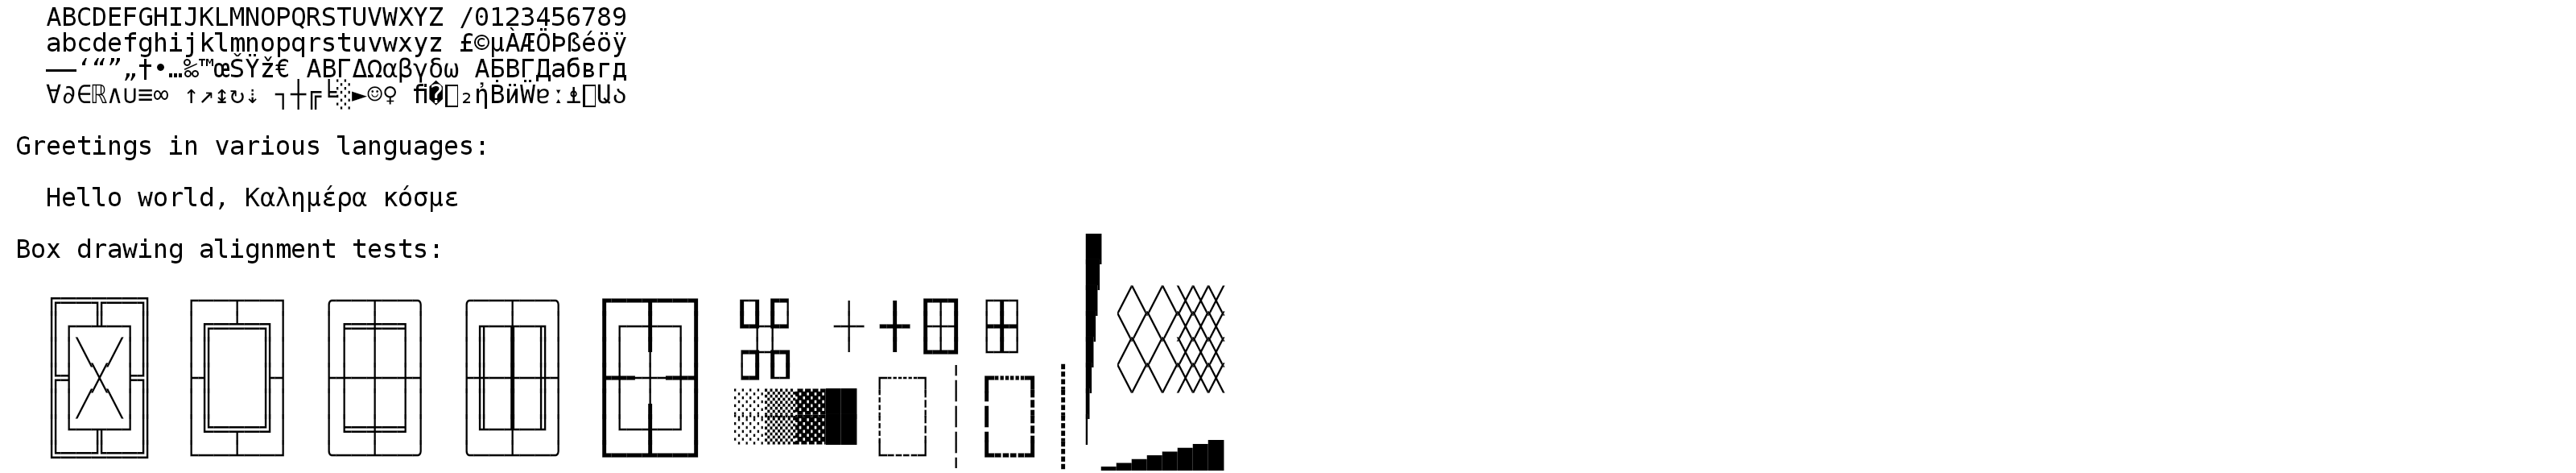
\includegraphics[width=0.9\linewidth]{graphics/utf8.png}
    \captionof{figure}[UTF8]{GLVisualize's fast UTF8 rendering with the help of Cairo, a texture atlas and 2D particles.}
    \label{fig:UTF8}
\end{minipage}

Vector graphics are difficult to render, as they are not a well fit for the \ac{GPU}.
Long stretched, curved and thin lines introduce several problems for the GPU\cite{Liland565821}.
Another problem is that splines used in vector graphics are usually supplied as Bézier curves, which are very demanding to rasterize.
Besides from that, anti-aliasing of thin lines introduces some problems as well. With post processing anti-aliasing techniques, lines which are thinner than one pixel will introduce artifacts, as OpenGL primitives smaller than a pixel will get discarded by the OpenGL pipeline. So additional care needs to be taken in order to assure, that primitives are always thicker than one pixel, or multi-sampling techniques have to be used.
This is only a very short summary of the problems, which is only given to illustrate that this is not a problem that can be solved in the scope of this thesis. 
Instead, FreeType[reference?!] is used for rendering fonts. As FreeType is relatively slow, these renderings get cached in a texture atlas from which they can get queried and rendered to the screen in large numbers.
This results in high quality and fast renderings. This comes at the cost of higher space requirements and resolution dependence.
So when zooming into the vector graphics, either a new version has to be rendered or one gets pixelated results.
In the future, distance fields can be used to reduce the resolution dependence\cite{Green:2007:IAM:1281500.1281665}.

\subsubsection{Volume Rendering}
\vspace{1em}
\begin{minipage}{\linewidth}
    \centering
    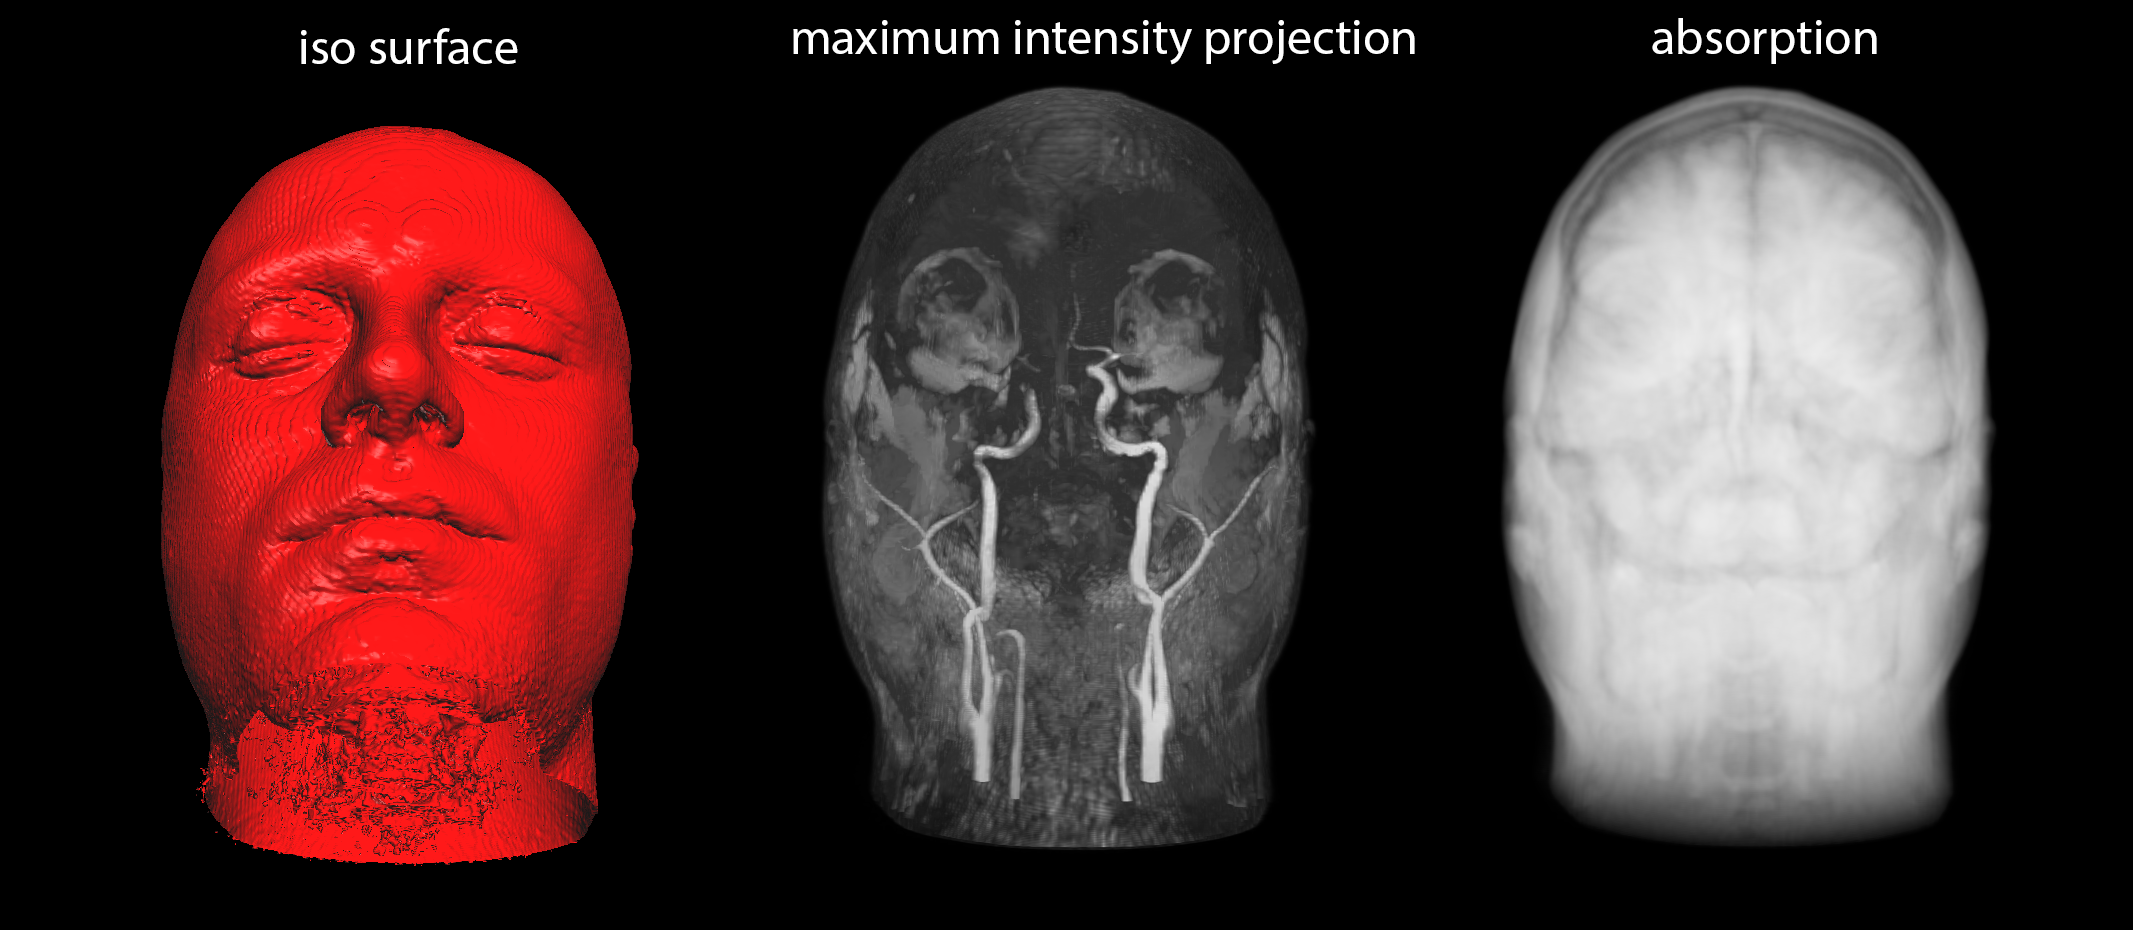
\includegraphics[width=0.9\linewidth]{graphics/volumes.png}
    \captionof{figure}[Volumes]{Different visualizations rendered with GLVisualize. As can be seen, every methods misses critical features of the volume.}
    \label{fig:volumes}
\end{minipage}

Volumes in 3D computer graphics are usually represented as voxels, which can be understood as 3D pixels. 
They represent values on a 3D grid. The name stems from the marriage of volume and pixel.
There are sparse and dense storage options for voxels and different informations can be represented, like speed, rotation, color, intensities and so forth.
Volume renderings are no trivial task. Not only from a computational point of view, but it is also difficult to make a visualization which lets you peek inside a volume without discarding important information. This is illustrated in figure \ref{fig:volumes}.
This is why different forms of visualizations are needed to get a good representation of a volume.
GLVisualize is able to render iso-surfaces, maximum intensity projections and an absorption based visualization form. 
On top of this, the particle systems can be used to give further insights into the volume by rendering particles for each voxel. This is especially helpful for sparse volumes, as these are not yet supported natively by GLVisualize.

For the Volume rendering two techniques are being used. 
Marching tetrahedra and ray casting\cite{marques2009gpu}. 
Marching tetrahedra is an algorithm that can be used to extract a mesh representation of an iso-surface from a volume.
Ray marching is the process of shooting rays from the camera origin through the object.
With every step inside the volume, values are sampled and depending on the combination of these values, different visualization forms can be realized. When you stop at a certain value, iso-surfaces can be rendered. 
If only the maximum is kept, it will yield a maximum intensity projection. 
When all values are combined via an absorption function, the volume will be displayed as if it is made of some translucent material like smoke.

The ray casting rendering method was explicitly implemented for this thesis on the GPU. For the marching tetrahedra algorithm there was already a Julia implementation available in the package Meshes.jl\cite{Tedrahedra}. The resulting mesh can be displayed with GLVisualizes mesh rendering capabilities.
Both techniques have their advantages and disadvantages. 
While marching tetrahedra is relatively slow, it can be used to generate a mesh which is very fast to display. 
Ray casting on the other hands allows for a wide range of visualization forms and is rather fast as it runs on the GPU. The downside is, that the calculation can not be cached camera position independent. But it allows to interactively change the iso values and all the other parameters, making it ideal to explore a volume.
 

\subsection{Scene Graph}
The scene graph is in the case of Romeo not a specialized data structure, but rather just a list of objects, which can be directly rendered with OpenGL. Functionality from Reactive, GLAbstraction, GLVisualize and GLWindow are involved in this. GLvisualize creates a renderable object with GLAbstraction, which will get pushed into a render queue in the screen from GLWindow. Everything that moves is handled via signals from Reactive.
Asynchronously updating the signals and iterating over the render object list is achieved with Julia's simple asynchronous API. It is not truly multi-threaded, but rather creates a producer-consumer structure. It can be multithreaded, but this is more difficult due to \ac{OpenGL} not being thread safe.
This is an extremely simple form of a scene graph, which does not allow to perform any optimizations.
Optimizations usually include sorting in order to reduce OpenGL state changes and culling of invisible objects.
As GLVisualize produces OpenGL code which relies only on very few calls to OpenGL, the first optimization is currently not as important.
But culling can make a large difference for big 3D scenes, as usually only a fraction needs to be rendered.
As this is a more involved process, which would preferably be done completely on the GPU, this was not in the scope of this thesis.

\subsection{3D Picking}

3D picking is the process of selecting a 3D object from a 2D projection like it is the case when you select a 3D object on the screen with the mouse.
It forms the basis for any mouse interaction with objects displayed on the screen.
The two most usual approaches are ray picking and color picking.
For the ray picking approach a ray is send from the 2D position of the camera plane into the 3D scene and is tested for intersection with every object in the scene. In contrast, color picking works with an extra render target, which stores an object id for every pixel, which gets written together with the color pass inside the fragment shader.
Color picking has been chosen for this thesis, as it is far easier to implement. Ray picking must be implemented on the GPU, best with some data structures optimized to do fast ray intersections. Otherwise, it will be very slow. If done on the CPU, the 3D objects need to be kept in video memory and CPU memory, further introducing complexity and bottlenecks.

For color picking, two frame-buffer render targets need to be created. 
One for the color channel and one to represent the object id plus an additional number to store contextual information. The additional number is usually used for the instance index, which can be used to e.g. infer what text glyph is selected.
When rendering, the fragment shader does not only write the color into the render target, but if the color is opaque also the current object id.
This way transparency aware 3D picking can be achieved without an extra processing step. 
The advantage of this methods is that one does not need an extra pass over the geometry. The disadvantage is higher space requirements and that OpenGL's native anti-aliasing does not work well together with the additional render target. Also, the OpenGL pipeline has to be flushed in order to read from the frame-buffer.
The anti-aliasing problem can be solved by implementing an extra anti-aliasing post processing step. A very simple FXAA algorithm has been implemented, which does not give perfect results but is fast and was easy to implement. The algorithm was taken from Matt DesLauriers\cite{FXAA} and was adjusted to fit into GLVisualiz's pipeline.


\subsection{Romeo}

So far Romeo just consists of one file with 500 lines of code. It just defines some simple text field, a search field, and a visualize and edit window.
The texts gets evaluated as Julia code as soon as it changes. Like this, the text field acts like a very simple \ac{REPL}.
Via the search field, you can execute simple Julia statements and the results will be displayed in the visualize window, while all parameters can be edited via the edit window.
This means, if you type in a simple variable, the variable will be visualized. But you can also search and transform a variable via simple Julia terms.
In \ref{app:screenshot} a screens shot of Romeo can be seen.
On the left is a window for editing scripts. The middle is used to visualize bound variables, in this case the variable \textit{barplot} is visualized.
On the bottom of the middle, the variables can be selected via a text field. The text field allows to execute code, so one can do things like filtering an array which then will displayed the filtered array.
On the right all variables of the visualization can be edited interactively.
If you click on the color circle for example, a color chooser will pop up which will let you chose the color.
The numbers are sliders, so when one clicks and drags on them, the value can be adjusted. 
While changing the values, the changes will be immediately displayed.



\section{Results and Analysis}
\section{Results and Discussion}

\subsection{Performance Analysis}
This chapter supplies some benchmarks, to analyze how close this thesis comes to achieve the wanted performance, which should be on eye level with C.

If not stated otherwise, benchmarks are written for this thesis and executed on an Intel Core i5-4200U with an HD 4400 graphic and 8GB of RAM.
Julia 0.4 has been used, C++ code hase been compiled with VS13 and for python the anaconda distribution with Python 2.7 was used.
Benchmarks were run on an idle computer with as little background processes running as possible.
The sources of the benchmarks can be found on Github.

\subsubsection{Julia}

Julia's performance is crucial for this thesis. 
If Julia does not perform close to C it would weaken the whole argument of writing the visualization library in Julia.
It is a very tedious task to write representative benchmarks for a programming language. 
The only way out is to rely on a multitude of sources and try to find analytical arguments.
In this thesis, Julia's own benchmark suite will be used in addition to some real world benchmarks.
In addition, the general compiler structure of Julia will be analyzed to find indicators for the limits of Julias performance.

\vspace{1em}
\begin{minipage}{\linewidth}
    \centering
    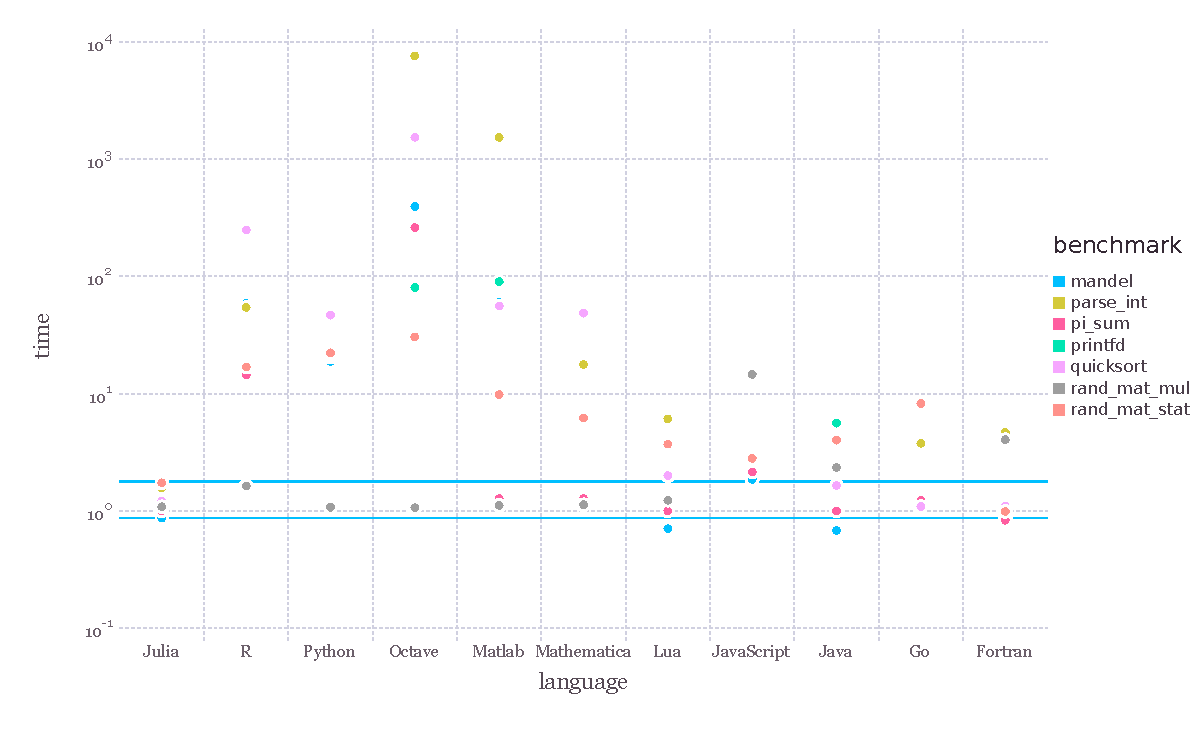
\includegraphics[width=0.9\linewidth]{graphics/juliabench.pdf}
    \captionof{figure}[Julia Performance]{Julia's performance compared to other languages, taken from Julia's micro bench suite \cite{JuliaBench}. Smaller is better, C performance = 1.0.}
    \label{fig:juliabench}
\end{minipage}

In the first benchmark from figure \ref{fig:juliabench}, we can see that Julia stays well within the range of C Speed. 
Actually, it even comes second to C-speed with no other language being that close.
This is a very promising first look at Julia, but it should be noted, that these benchmarks are written by the Julia core team.
So it is not guaranteed, that there is no bias favoring Julia in these benchmarks.
There is another benchmark comparing C++, Julia and F\#, which was created by Palladium Consulting which should not have any interest in favoring one of the languages.
They compare the performance of C++, Julia and F\# for an IBM/370 floating point to IEEE floating point conversion algorithm. This is part of a blog series\cite{JuliaFSCpp} written by Palladium Consulting.
F\# comes out last with 748.275 ms, than Julia with 483.769 ms and finally C++ with 463.474 ms. 
At the citation time, the Author had updated the C++ version to achieve 388.668 ms. 
It looks like the author was only working on making the C++ version faster, so it can not be said that the other versions could not have been made faster too.


The last Julia benchmark is more real world oriented. 
It is comparing Finite Element solver, which is an often used algorithm in material research and therefore represents a relevant use case for Julia.

\begin{table}[htbp]
    \centering
    \begin{tabular}{l|c|c|c}
        \hline
        \textbf{N}  & \textbf{Julia} & \textbf{FEniCS(Python + C++)}  & \textbf{FreeFem++(C++)}\\
        \hline
        121         & 0.99           & 0.67             & 0.01 \\
        2601        & 1.07           & 0.76             & 0.05 \\
        10201       & 1.37           & 1.00             & 0.23 \\
        40401       & 2.63           & 2.09             & 1.05 \\
        123201      & 6.29           & 5.88             & 4.03 \\
        251001      & 12.28          & 12.16            & 9.09 \\
        \hline
    \end{tabular}
    \captionof{table}[FEM Benchmark]{Performance of a FEM solver written in Julia compared to some existing libraries. \cite{FMSolver}}
    \label{table:fembench}
\end{table}
These are remarkable results, considering that the author states it was not a big effort to achieve this. After all, the other libraries are established FEM solvers written in C++, which should not be easy to compete with.

This list could go on, but it is more constructive to find out Julia's limits analytically.
As already mentioned, Julia is statically compiled at runtime. This means, as long as all types can be inferred at runtime, Julia will have in the most cases identical performance to C++.
The biggest remaining difference in this case is the garbage collection. Julia 0.3 has a mark and sweep garbage collector, while Julia 0.4 has an iterative mark and sweep garbage collector.
As seen in the benchmarks, it does not necessarily introduce big slowdowns.
But there are issues, where garbage collection introduces a significant slow down\cite{ReadDlmGC}.
Analysing this further is not in the scope of this thesis, though. 
But it can be said that Julia's garbage collector is very young and only the future will show how big the actual differences will be.

Another big difference is the difference in between different compiler technologies.
\ac{LLVM}'s biggest rival is \ac{gcc}. If C++ code that is compiled with \ac{gcc} is much faster than the same code compiled with \ac{LLVM}, the \ac{gcc} version will also be faster as a comparable Julia program.
In order to investigate the impact of this, one last benchmark will be analyzed.
This is a summary of a series of articles posted on Phoronix, which benchmarked \ac{gcc} 4.92 against \ac{LLVM} 3.5 and \ac{LLVM} 3.5 against \ac{LLVM} 3.6:
\begin{table}[ht]
  \centering
  \begin{tabular}{l|c|c}
    \hline
    \textbf{Method} & \textbf{\ac{gcc} vs \ac{LLVM} 3.5} & \textbf{\ac{LLVM} 3.5 vs \ac{LLVM} 3.6} \\
    \hline
    mean & 0.99 & 0.99 \\
    median & 0.97 & 1.00 \\
    maximum & 1.48 & 1.10 \\
    minimum & 0.39 & 0.88 \\
    \hline
  \end{tabular}
    \captionof{table}[gcc vs llvm summary]{Summary of the Phoronix benchmark. Unit is speedup of LLVM, bigger is better. \cite{LLVM35vsLLVM36}\cite{LLVMvsGCC}\cite{Phoronix}}
    \label{table:gccvsllvm}
\end{table}

The full tables can be found in the appendix under the table \ref{table:llvm35vsllvm36} and \ref{table:llvmvsgcc}.
The results suggest, that \ac{LLVM} is well in the range of \ac{gcc}, even though that there can be big differences between the two.
These are promising results, especially if you consider that LLVM is much younger than gcc. 
With big companies like Apple, Google\cite{GoogleAppleLLVM} and Microsoft\cite{MicrosoftLLVM} being invested in LLVM, it is to be expected that \ac{LLVM} will stay competitive, which means Julia should in theory stay competitive as well.


\subsubsection{ModernGL}
\vspace{1em}
\begin{minipage}{\linewidth}
    \centering
    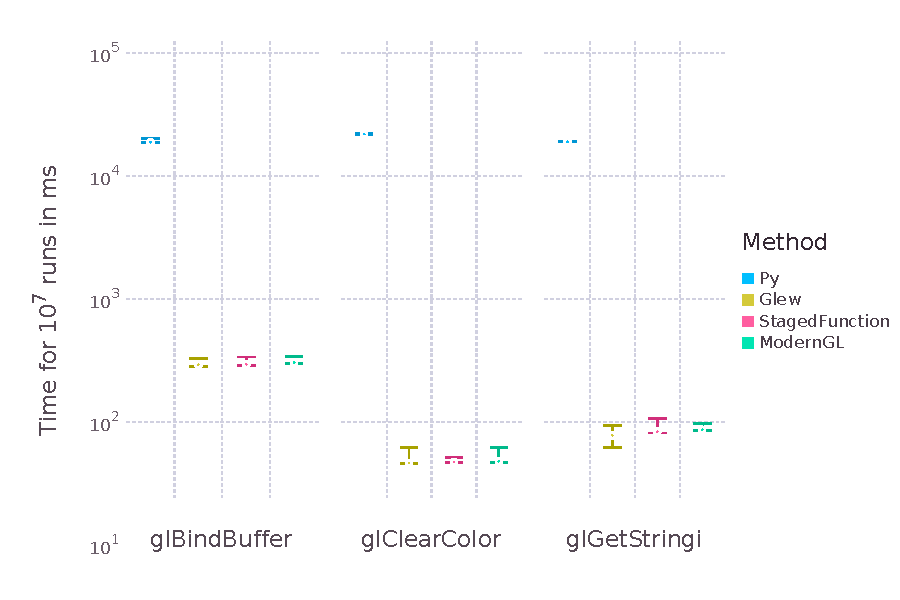
\includegraphics[width=0.9\linewidth]{graphics/glbench.pdf}
    \captionof{figure}[OpenGL Wrapper]{Different performance of OpenGL wrappers. The time for $10^7$ calls was measured 100 times for each function.}
    \label{fig:openglwrapper}
\end{minipage}
\begin{table}[htbp]
    \centering
    \begin{tabular}{l|c|c|c}
        \hline
        \textbf{Function}   & \textbf{Python}    & \textbf{Staged Function} & \textbf{ModernGL} \\
        \hline
        glBindBuffer        & 64.43              & 1.00 & 1.04 \\
        glClearColor        & 474.72             & 1.02 & 1.04 \\
        glStringi           & 244.44             & 1.07 & 1.1  \\
    \end{tabular}
    \captionof{table}[OGL Relative Speed]{Performance relative to C++ with Glew (slowdown, bigger is worse)}
    \label{table:relativespeedoglw}
\end{table}

In this chapter, ModernGL, GLEW and PyOpenGL will get benchmarked.
The procedure was, to call an OpenGL function $10^7$ times in a tight loop. Execution time of the loop gets measured.
The results are plotted in figure \ref{fig:openglwrapper}.
ModernGL seems to do pretty well compared to C++ and python does very badly, with being up to 470 times slower in the case of glClearColor.
Julia in contrast offers nearly the same speed as calling OpenGL functions from C++ as can be seen in the table \ref{table:relativespeedoglw}.
As all the OpenGL wrappers are pretty mature by now and bind to the same C library (the video driver), this should mainly be a C function call benchmark.
Python performs badly here, but it must be noted that there are a lot of different Python distributions and some promise to have better C interoperability.
As this benchmarks goal is to show that Julia’s ccall interface is comparable to a C function call from inside C++, the python options have not been researched that thoroughly.
From this benchmark can be concluded, that Julia offers a solid basis for an OpenGL wrapper library.


\subsubsection{Reactive}

\begin{figure}
\centering
    \begin{minipage}{.5\textwidth}
        \centering
        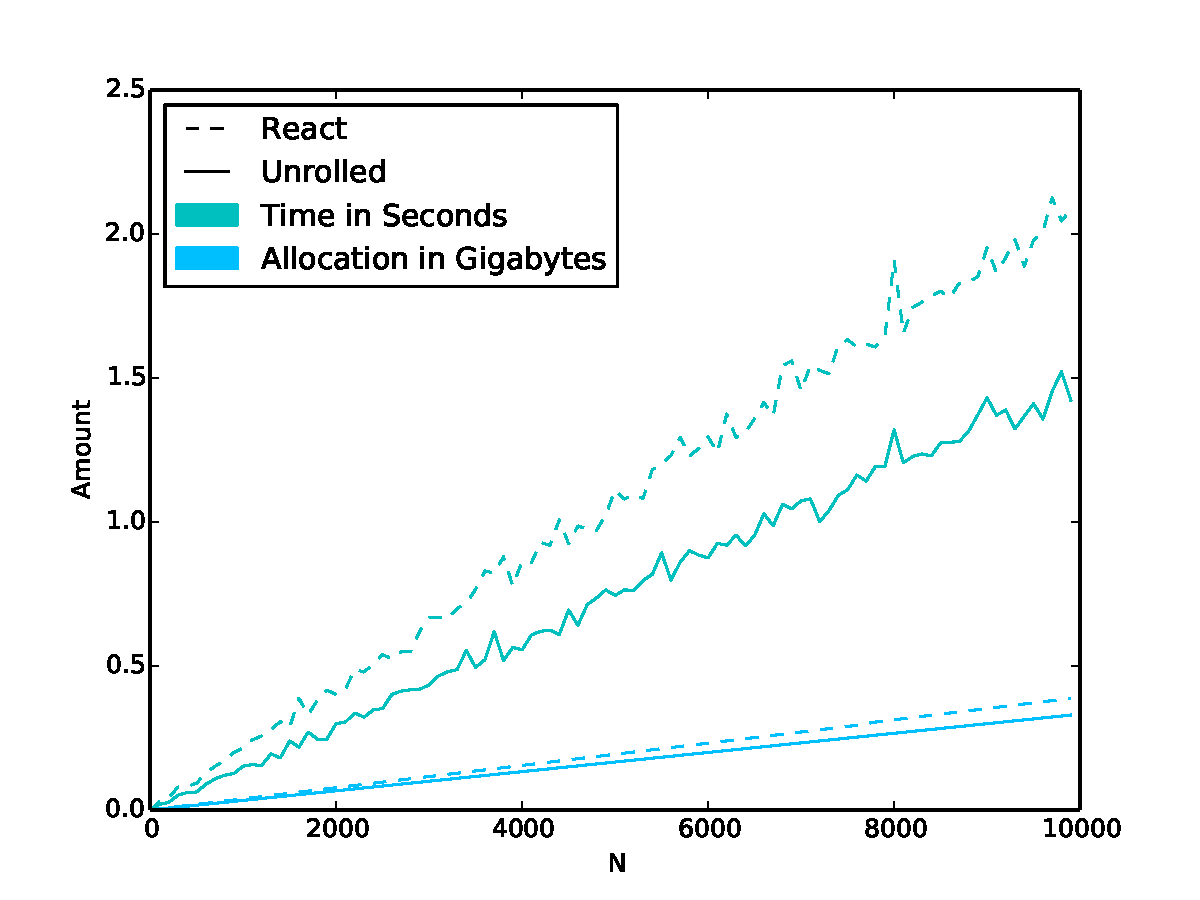
\includegraphics[width=0.9\textwidth]{graphics/react_bench_2.pdf}
        \captionof{figure}[Reactive 1]{Complicated graph, simple calculation}
        \label{fig:reactive1}
    \end{minipage}%
    \begin{minipage}{.5\textwidth}
        \centering
        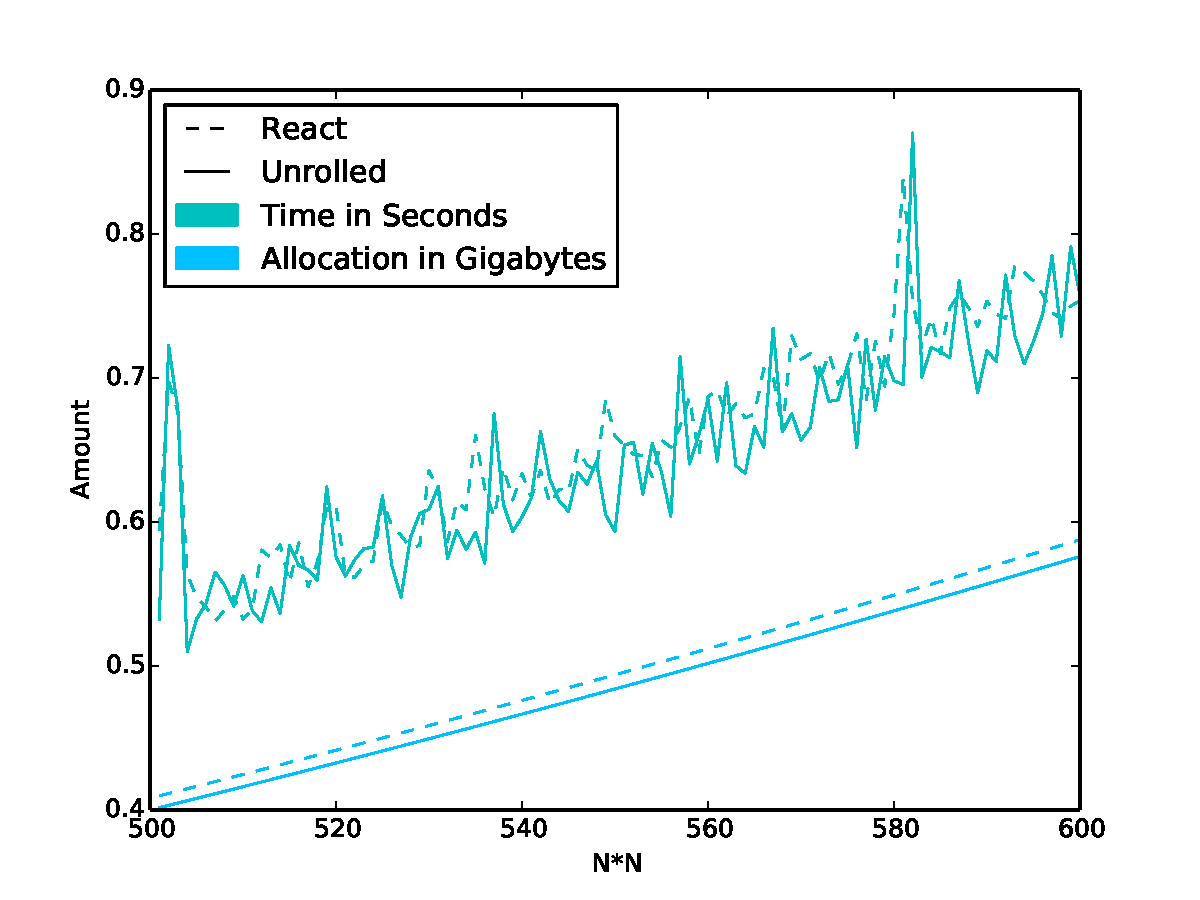
\includegraphics[width=0.9\textwidth]{graphics/react_bench_1.pdf}
        \captionof{figure}[Reactive 2]{High memory, simple event graph}
        \label{fig:reactive2}
    \end{minipage}
\end{figure}

It is relatively hard to benchmark the used event system in real world scenarious as it is hard to find a baseline.
One would have to rewrite Romeo with another Event system. 
Using other visulization libraries as a baseline is also difficult, as it is hard to isolate the performance of the event system.
This is why we will compare an event graph from Reactive with its unrolled version.
For the unrolled version the functions from the callback graph have been executed in the same order as the event graph would have without introducing any event system related overhead.
This way we can measure the overhead introduced by the event system.
Two code samples have been benchmarked, one simulating the operation needed for the camera and the other simulates animating a large array.
The first has low memory usage with a more complex event graph. The second has a straight forward event graph, but it must pass on a large array and needs to execute the callbacks on the array.

As can be seen in figure \ref{fig:reactive1}, small operations with a complex event graph has some noticable overhead. Reactive is in this scenario about 1.45 times slower than the optimal version.
This does not come as a surprise as sorting and managing the graph structure obviously adds some overhead.

The second scenario looks much better for Reactive. The performance difference is neglectable, making Reactive a good choice for creating signals with high memory throughput.

\subsubsection{3D Rendering Benchmark}

\begin{minipage}{\linewidth}
    \centering
    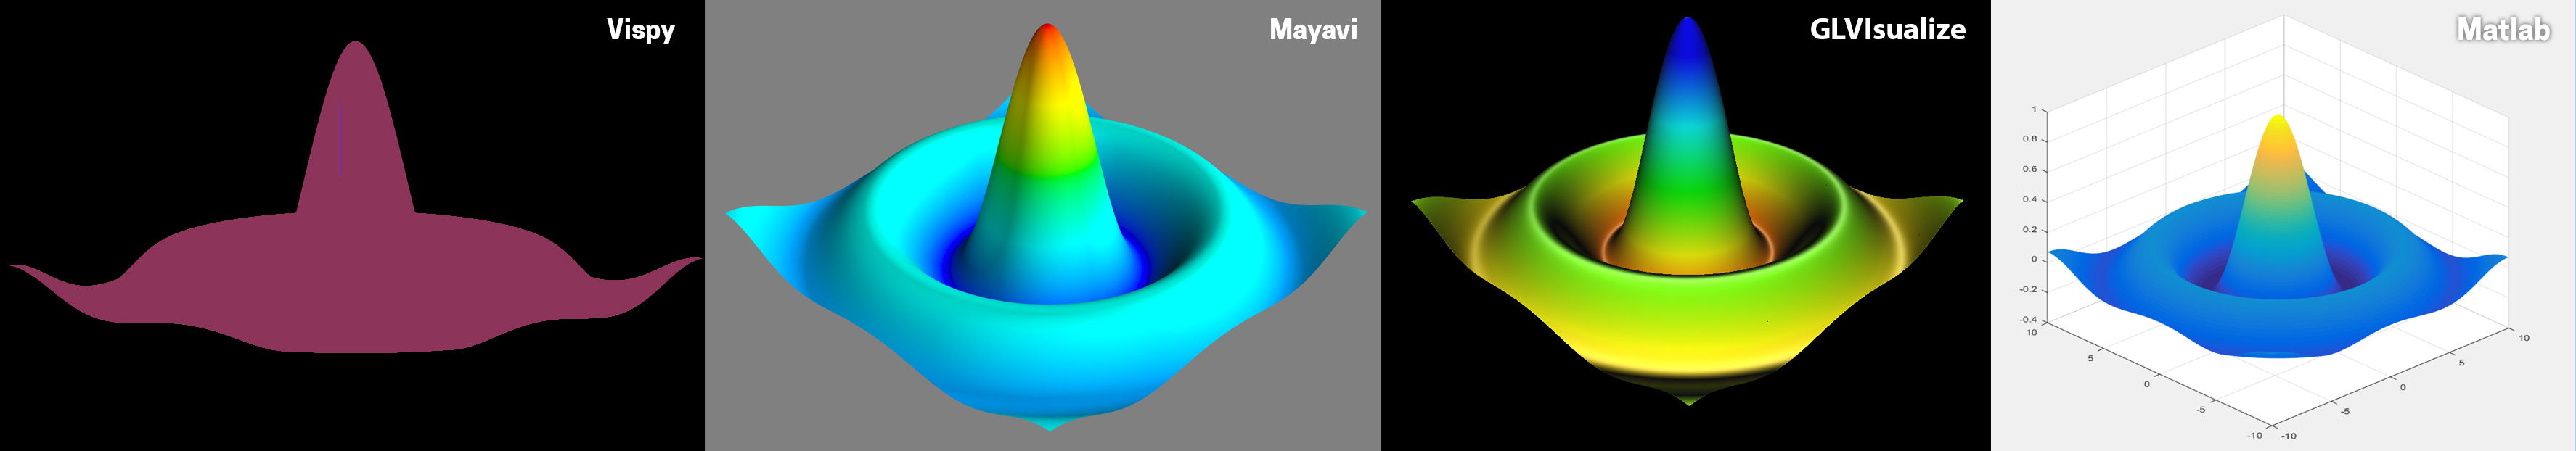
\includegraphics[width=\linewidth]{graphics/vispy_mayavi_romeo.jpg}
    \captionof{figure}[Benchmark]{Different visualizations of the same surface}
    \label{fig:reactive1}
\end{minipage}

The biggest problem with benchmarking the 3D rendering speed is, that there is no library which will allow to exactly reproduce similar conditions and measures. 
Additionally, without extensive knowledge of the library, it is difficult to foresee what gets benchmarked. 
As an example of why it is difficult to measure the frame rate we can look at Vispy. When you enable to measure the frame rate, it will show very low frame rates, as it only creates a new frame on demand.
On the other side Romeo has a fixed render loop, which renders as much frames as possible, leading to totally different amount of rendered frames per second. 
This is why it was decided, to use the threshold at which a similar 3D scene is still conceived as enjoyable and interactive. Usually the minimal amount of frames per second for perceiving movements as smooth is around 25.
So the benchmark was executed in the way, that the number regulating the complexity of the 3D scene was increased until one could not move the camera without stutters. The recorded threshold is than the result of the Benchmark.

First benchmark is an animated and still 3D surface plot. The libraries offering this functionality where Vispy, Mayavi and Matlab.

\begin{table}[htbp]
    \centering
    \begin{tabular}{l|l|l}
        \hline
        \textbf{Library} & \textbf{Still} & \textbf{Animated} \\
        \hline
        Vispy            & 300            & 80    \\
        Mayavi           & 800            & 150   \\
        Matlab           & 800            & 450   \\
        Romeo            & 900            & 600   \\
        \hline
        \hline
        Speed up Vispy   & 9x            & 56x   \\
        Speed up Mayavi  & 1.26x         & 16x   \\
        Speed up Matlab  & 1.26x         & 1.7x  \\
    \end{tabular}
    \captionof{table}[3D Benchmark]{3D surface created from a NxN matrix.}
    \label{table:relativespeedoglw}
\end{table}
Vispy had some issues, as the camera was never really smooth for the surface example. Also the normals were missing and there was no option to colorize the surface depending on the height.
It was decided to use the threshold of going from a little stutter to unpleasant stutters, making vispy not completely fail this benchmark.
For Vispy it was found out, that the normals where calculated on the CPU resulting in a major slow down\cite{VispyGithub}. The same can be expected for Mayavi, but Mayavi seems to be faster at calculating the normals.
There is not much information available on how Matlab renders their visualization, as it is closed source.

\begin{minipage}{\linewidth}
    \centering
    \includegraphics[width=\linewidth]{graphics/romeo_mayavi_particles.jpg}
    \captionof{figure}[Particles]{Rendered particles}
    \label{fig:reactive1}
\end{minipage}

The next benchmark is only between Romeo and Mayavi, as the other libraries did not offer a comparable solution. Matlab does not allow to use cubes as particle primitives and Vispy only had an example, where you needed to write your own shader, which can not be seen as a serious option. This is a benchmark for easy to use and high level plotting libraries. It is always possible to write an optimal version yourself in some framework, but what really interesting is, how well you can solve a problem with the tools the library has readily available.

\begin{table}[htbp]
    \centering
    \begin{tabular}{l|l|l}
        \hline
        \textbf{Library} & \textbf{Still}  & \textbf{Animated}  \\ 
        \hline
        Mayavi           & 90000           & 2500  \\
        Romeo            & 1000000         & 40000 \\
        \hline
        \hline
        Speed up         & 11x             & 16x \\
    \end{tabular}
    \captionof{table}[3D Benchmark]{Maximum number of particles that could be displayed without stutter.}
    \label{table:relativespeedoglw}
\end{table}
Romeo is an order of magnitude faster in this specific benchmark. This is most likely due to the fact that Romeo uses OpenGL's native instance rendering.


\subsubsection{IJulia}

It was not possible to compare IJulia directly with Romeo, as the feature set for plotting is too different.

But there are certain factors, which indicate, that is hard to reach optimal performance with IJulia.
First of all, IJulia uses ZMQ to bridge the web interface with the Julia kernel.
ZMQ is a messaging system using different sockets for communication like inproc, IPC, TCP, TIPC and multicas.
While it is very fast at it's task of sending messages, it can not compete with the native performance of staying inside one language.
This is not very important as long as there does not have to be much communication between Julia and the IPython kernel. This changes drastically for animations, where big memory chunks have to be streamed to the rendering engine of the browser. It can be expected, that this will always be a weakness of IJulia.
On the other hand, GPU accelerated rendering in a web browser is also limited.
It relies on WebGL, which offers only a subset of the OpenGL's functionality. So while the execution speed of OpenGL can be expected to be similar, there are a lot of new techniques missing, which can speed up rendering.

To investigate this another benchmark has been created.
It is between Romeo and Compse3D, which was the only library found to be able to display 3D models created with Julia directly from the IJulia notebook.
This benchmark is not entirely fair, as Compose3D is just a very rough prototype so far. 
But there seems to be no other library with which you can easily create and display interactive 3D graphics in the IJulia or IPython notebook. 
This benchmark creates a sierpinsky gasket and Compose3D displays it in the IJulia notebook while Romeo displays it natively in a window.

\begin{minipage}{\linewidth}
    \centering
    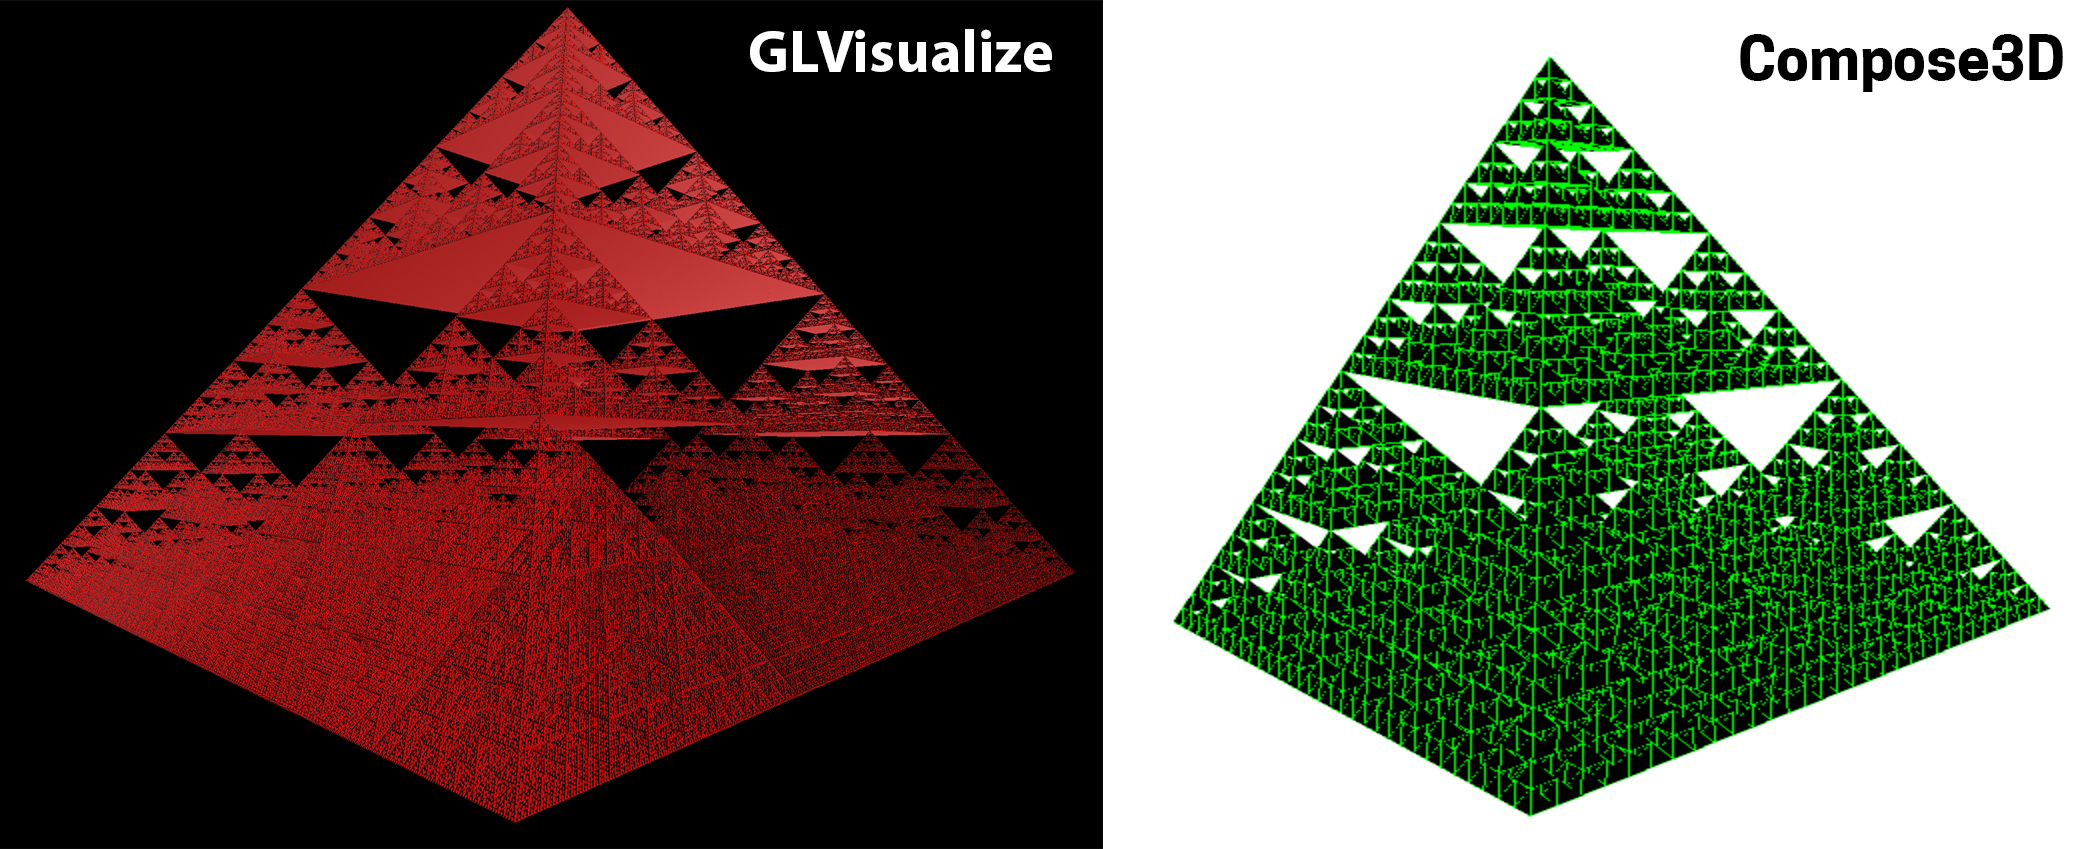
\includegraphics[width=\linewidth]{graphics/sierpinsky.jpg}
    \captionof{figure}[Sierpinsky]{Sierpinsky pyramid in 3D}
    \label{fig:reactive1}
\end{minipage}
\begin{table}[htbp]
    \centering
    \begin{tabular}{l|l}
        \hline
        \textbf{Library} & \textbf{Still}\\ 
        \hline
        Compose3D        & 15625         \\
        Romeo            & 1953125       \\
        \hline
        \hline
        Speed up         & 125x          \\
    \end{tabular}
    \captionof{table}[3D Benchmark]{Maximum number of pyramids that could be displayed without stutter.}
    \label{table:relativespeedoglw}
\end{table}

Again, Romeo is an order of magnitude faster. This can change in the future when Compose3D matures.
But one needs to notice, that Romeo utilizes OpenGL's instancing to gain this speed. Native instancing is not yet available in WebGL, which means that this optimization will not be available for the IPython notebook in the near future.

\subsection{Extensibility Analysis}

The modular design of Romeo has proven to be effective and the goal of re-usability has already proven itself.
Most of the created modules are used independently by different people.
GLVisualize is used by myself for two packages, namely GLPlot, a scientific plotting package for Julia and for a prototype of a file explorer.
It got forked by several users to create their own dynamic visualization packages.
The same applies for ModernGL and GLAbstraction. Most other used packages are at least used by one other project.
This indicates, that the abstraction and modularity is well designed, so that all the modules can function on their own.

The only exception is GLWindow, which has been used just indirectly through the other packages. 
This can mean three things.
First, it is badly abstracted and does not cleanly wrap one use case.
Secondly, it can be that the use case is not entirely clear to other people, which would not be a big surprise considering the minimal amount of documentation for GLWindow.
And finally, considering the small group of people developing graphics for Julia, it could be that they simply do not need the lower level functionality of GLWindow and instead rely on the other written packages that use GLWindow.

Modularity guarantees a broad user and developer base, which in turn results in rich functionality and stability.
From further analyzing the Github repository written for this thesis, one can find out that there is a general lack of documentation.
This hinders people from contributing and using the packages.

The implementation in just one language has been achieved by choice. There are only a few exceptions, like the kernel code for OpenGL shaders, which currently can not be written in Julia. 
Julia programmers that use Romeo can extend Romeo with Julia and immediately see their results without complicated compilations.
This together with the speed is one of the main achievements compared to other libraries offering similar functionality, like IJulia, Mayavi and Matlab.
To further proof this point I will analyze the mentioned software in more detail.
The language usage statistics and necessary tools needed in order to extend the software will be the main focus of the analysis.
One needs to note, that the usage statistic of languages is just a weak indicator for the extendability of a software.
Using different languages for one project can make sense if the project has different domains where domain specific languages give an advantage. As this means one needs to know all used languages, this still introduces complexity, but it is at least justified complexity.
This chapter will only discuss the complexity introduced by languages, which are only needed for compatibility with other libraries or because the main language is too slow. This is something, which should ideally be avoided.


\subsubsection{IJulia}

IJUlia is written in Julia and relies on ZMQ(C++) and IPython. 
IPython uses multiple JavaScript rendering back ends like Three.js and D3.
\begin{table}[htbp]
    \centering
    \begin{tabular}{l|l}
        \hline
        \textbf{Software} & \textbf{languages used}\\
        \hline
        IPython     & Python 78.5\% JavaScript:15.1\% HTML 5.0\% Other 1.4\%\\
        Three.js:   & JavaScript 62.4\% HTML 26.4\% Python 6.9\% C++ 1.9\% C 1.3\% GLSL 0.6\%\\
        D3:         & JavaScript 95.6\% CSS 4.3\%\\
        \hline
        \end{tabular}
    \captionof{table}[IJulia Stack]]{Technologies used in IJulia. Statistics taken from Github}
    \label{table:ijuliastack}
\end{table}
[more to come]

\subsubsection{Mayavi and VTK}

Table \ref{table:ParaviewStatistic} in the appendix shows an extensive summary of the used languages in the Paraview repository.
It amounts to a total of 3.642.105 lines of code written in 29 languages.
[more to come]

\subsubsection{Matlab}

Matlab is closed source, which makes the core of Matlab impossible to extend by the user.
This is why Matlab relays on a plug-in architecture, which enables developers to write closed or open source plug-ins for Matlab.
[Analysis of the plug-in Architecture]
[more to come]


\subsection{Usability Analysis}
%Consistency and ease of use of programming API in GLVisualize+GLAbstraction and Romeo.
%Short comment about the \ac{GUI}
Doing a broad user survey or similar methods was out of scope for this thesis.
As a result from this, the usability study has to be done analytically.
There are different aspects which can be analyzed. For example, how many function names need to be remembered, how easy they are memorized, if they expose the wanted functionality and how difficult it is to look up unknown functionality.
For this thesis, I will analyze the two main packages, namely GLVisualizes and GLAbstraction. 
The named aspects will be analyzed and in addition feedback from Github will be used.

GLVisulize has a very simple API, as it offers only five functions: visualize, visualizedefaults, edit and renderloop.
There are also the functions bounce and loop, which offers a simplification for creating periodic signals.
These functions might get moved into Reactive, though.
So for GLVisualize, only very few function names have to be remembered.
The question is, does this simple interface still allow people to create the visualization they want.
At closer inspection one can see, that visualize is overloaded 67 times, with each of these methods having a set of keyword arguments which enables further customization.
These can introduce drastic changes. The particle visualization for example can take any mesh as a primitive. This enables a customization, which was not possible in such an easy way in the other examined packages.
Also, most of the functions take either a data type, or a signal of that data type.
This makes it very intuitive to animate your data. 
In contrast, in order to setup the animation for the other packages, it took quite some time to find out how to update values of an existing visualization. This is acceptable, as it might take quite some time to find out that Romeo uses signals and how to work with signals.
But when this is found out, Romeo functions in the same, consistent way. Signals add a fourth dimension to any parameter or data you would like to visualize, making the usage principle consistent across the different visualizations.

For the other packages though, one needs to find out the names of the data for every visualization type in order to access and update them. Some attributes can not be animated, making the API even less consistent.

So for Romeo one can achieve anything by bringing the data into the right format.
Problems arise, if this can not be done easily or the format is not intuitive for the programmer.
To be fair, you will have this problem with every kind of visualization API. 
The difference is in the end, how easy it is to do the data transformations. 
Lets examine an example, where GLVisualize often will not allow to directly call visualize on the data.
There is only a method for visualizing a Mesh, but not for a vertex list plus a face list. If you work with mesh data, you will often handle the face and vertex list isolated.
So an API that offers a function like \texttt{visualize\_mesh(x::VertexList, y::FaceList)} will be more straightforward for a programmer.
Especially, as this is the standard way of displaying a mesh in most scientific plotting packages. This has become one of the most occurring questions on github, even though that there are usage examples for displaying a mesh.

But this functionality can be added in a simple way for GLVisualize by defining \texttt{visualize\_mesh(facelist, vertexlist) = visualize(Mesh(facelist, vertexlist))}.
As GLVisulize should stay as close to the principle of only having one function name, this should be moved to other interface only packages, though.
[more to come]

\section{Conclusion}
\section{Conclusion}

In this work, a fast 3D visualization library for scientific computing has been presented. 
The library's focus is not only speed but also usability and reusability. 
This is why some drastic design choices were made.
One of the most important ones was to write the library in Julia. 
This is a risky decision as Julia is a very young language, which is still in the alpha release phase. 
Because of this, there are not as many IDE's readily available, the language is still in flux, debugging is harder and the packages are not that mature and stable as in older languages.
Beside these problems, Julia turned out to be surprisingly stable and well suited for the task.
Using Julia brought the huge advantage of writing in a high-level language without sacrificing speed. 
That the advantages of Julia play out can be seen in the analysis chapter. It turns out that the developed packages offer state of the art speed, while being easy to use and extendable. 
This is mostly thanks to Julia and a modular design, which made it possible to write the whole visualization library with very little code, making it easy to overlook and reducing complexity. 
A simple interface for creating animated and interactive visualizations has been implemented by relying on signals for all data involved in the visualization.
It makes it very easy to animate every parameter of the visualization while keeping a concise code base.
Together with the edit widgets, GLVisualize enables users to change all parameters of a visualization interactively. 
This is used by Romeo to create an interactive scripting environment which enables people to execute scripts and visualize and interact with the variables.
The fact that it was possible to also implement other software packages like the chat client Osmosis along Romeo with only little effort are proof that the chosen abstractions and interfaces function well.
To enable more people to extend Romeo or create other libraries building upon GLVisualize a lot more work has to be done. 
One important first step is to improve the documentation. 
Also, the dependencies are difficult to install on some platforms. This indicates that a lot more testing and bug fixing needs to be done in order to create a pleasant user experience.
The rendering speed turned out to be very competitive compared to other established packages, but there is still more room for improvement.
More complicated benchmarks with complex scenes have not been benchmarked and it will be interesting to see if there will be large performance drops due to the simple scene graph that does not do any higher level optimizations yet.
As multithreading is not yet implemented, severe issues turn up when a task is computational heavy. This scenario will currently result in a freeze of the whole application. This is definitely not acceptable for a serious visualization library.
 
All in all, it has been shown that Julia and Romeo build a steady foundation for scientific projects with the need for highly performant and interactive 3D graphics.

\subsection{Future Work}

As already mentioned, there is a lot to do in order to make all packages more pleasant to use.
The scene graph is very simple, there is no real multithreading support, the anti-aliasing is sub-optimal, a lot of important features are missing and the OpenGL version used is just mildly modern, compared to the features recently released. 
Staying state of the art will be a big challenge, especially while keeping downward compatibility for platforms that do not support the newest feature set.
One of the most exciting possibilities though is to make parts of Julia compile to the GPU directly. 
This becomes possible, as the Khronos Group recently released \ac{SPIR-V}, an intermediate representation which \ac{OpenGL} and \ac{OpenCL} can compile to in the future. The Khronos Group plans to release a converter from \ac{LLVM} \ac{IR} to \ac{SPIR-V}, which would make it possible to program \ac{OpenGL} and \ac{OpenCL} alike functionality in any \ac{LLVM} based language\cite{SpirV}.
This means, that all the code that is currently written in \ac{GLSL} could be rewritten in Julia. 
On top of that, some functionality that is currently written in Julia and runs on \ac{CPU} could in the future be run on the \ac{GPU}. This includes functionality which would profit from highly parallel execution, like ray picking, calculating normals and culling objects.
This would further unify the platform, improve speed and will lower the complexity of the library. 
Such a unique feature is currently not implemented in any other language and could be a game changer for high performance visualization libraries.
With possibilities like these, one can look forward to a bright future for high performance graphics in Julia.


\nocite{*}

% ----------------------------------------------------------------------------------------------------------
% Literatur
% ----------------------------------------------------------------------------------------------------------
\renewcommand\refname{Bibliography}
\bibliographystyle{myalpha}
\bibliography{bibo}

\pagebreak

% ----------------------------------------------------------------------------------------------------------
% Appendix
% ----------------------------------------------------------------------------------------------------------
\pagenumbering{Roman}
\setcounter{page}{1}
\lhead{Appendix \thesection}

\begin{appendix}
\section*{Appendix}
\phantomsection
\addcontentsline{toc}{section}{Appendix}
\addtocontents{toc}{\vspace{-0.5em}}

\section{GUI}
A nice Appendix.

\subsection*{Screenshot}
\label{app:screenshot}
Category not in the table of contents.

\end{appendix}



\newpage
\thispagestyle{empty}
\begin{center}
	\vspace*{5em}
	\huge\textbf{Official Statement}\\
\end{center}
\vspace{2em}

I hereby guarantee, that I wrote this thesis and didn't use any other sources and utilities than mentioned.

\vspace{4em}
\begin{minipage}{\linewidth}
	\begin{tabular}{p{15em}p{15em}}
		Date: &  .......................................................\\
		& \centering (Signature)\\
	\end{tabular}
\end{minipage}

\end{document}